\chapter{Number Systems}
\markboth{Number Systems}{Number Systems}

\begin{remark}[Positioning of this chapter]\label{rem:chapter_positioning_ch2}
Number systems are the level-by-level realisation of the algebraic closure required for period determination. This chapter does not enumerate number systems from the standpoint of an `encyclopaedia of mathematical structures'; rather, it starts from the \textbf{requirements of period determination} and answers one core question: \textbf{for each class of periodic orbit to become a mathematically decidable object, what kind of number system is required as its algebraic foundation?}

The main line of logic is:
\[
\text{period determination requirement} \;\Longrightarrow\; \text{required algebraic closure} \;\Longrightarrow\; \text{number-system extension}.
\]

Each step of extension is driven by an \textbf{undecidable period problem} in the preceding number system. Each section answers three questions: which period is being determined? What was missing from the original number system? What criterion is obtained after the extension?

\textbf{Core insight: the hierarchical progression of transformations}. Repeated addition (translation) produces multiplication (scaling); repeated multiplication (scaling) produces powers (rotation). This hierarchical progression is the intrinsic driving force of number-system extension.

\textbf{The function-equation main line}. This chapter starts not only from the `requirements of period determination' but also from the `solvability of function equations'. The three function equations given in the preceding chapter---
\[
\text{Translation:} f(x+a)=f(x),\qquad
\text{Scaling:} f(qx)=f(x),\qquad
\text{Rotation:} f(e^{i\theta}z)=f(z)
\]
as well as the antiperiod equation $f(x+a)+f(x)=0$ (equivalent to $f(x+a)=-f(x)$)---
their solvability in each level of number system, and the structure of their groups with periodic orbits, constitute the other main line of number-system extension. Each level of number-system extension makes exactly one class of function equation pass from `unsolvable' or `non-closed' to `solvable', with its group with periodic orbits becoming a group. This line runs in parallel with the main line of `requirements of period determination', and together they drive the extension of the number systems from $\mathbb N$ to $\mathbb H$.

\textbf{Seven-theme guide to this chapter}: translation---the translation group $(\mathbb{Z},+)$ of the integers $\mathbb{Z}$ and its additive symmetry (centre of symmetry $0$); scaling---the proportional direction of the rationals $\mathbb{Q}$ and the multiplicative symmetry $\sigma_1$ (centre of symmetry $1$); rotation---the unit circle $U(1)$ of the complex numbers $\mathbb{C}$ and the $SU(2)$ three-dimensional rotation of the quaternions $\mathbb{H}$; conservation---the conserved quantities corresponding to the operations closed by each successive extension of the number systems (addition, multiplication, completeness, algebraic closure, non-commutative multiplication), namely momentum, phase volume, angular momentum and three-dimensional angular momentum; symmetry---the centres of symmetry $0$, $1$, $i$ emerging level by level as inverse operations are introduced; closure---the closure of the operations of each number system and the closure criterion for finite rotation orbits; period---the period types corresponding to the number systems (discrete translation period, finite rotation period, quasi-period, double period, three-dimensional rotation period).
\end{remark}

\section{\texorpdfstring{The natural numbers $\mathbb{N}$: counting and repetition, but not constituting a period}{The natural numbers N: counting and repetition, but not constituting a period}}

\subsection{\texorpdfstring{Determination requirement}{Determination requirement}}

The numbering of `the $k$-th element' in a periodic sequence, and the counting of `repeating $n$ times'.

\subsection{\texorpdfstring{The axiomatisation of the natural numbers}{The axiomatisation of the natural numbers}}

\begin{axiom}[Peano arithmetic]\label{ax:peano}
The number system of the natural numbers $\mathbb{N}$ is characterised by the following five axioms:
\begin{enumerate}[label=(\arabic*)]
    \item $0 \in \mathbb{N}$.
    \item Every natural number $n$ has a unique successor $S(n) \in \mathbb{N}$.
    \item $0$ is not the successor of any natural number.
    \item The successor function is injective: if $S(n) = S(m)$, then $n = m$.
    \item \textbf{The induction axiom}: if a subset $A \subseteq \mathbb{N}$ satisfies $0 \in A$ and $S(n) \in A$ for every $n \in A$, then $A = \mathbb{N}$.
\end{enumerate}
\end{axiom}

\begin{definition}[Operations on the natural numbers]\label{def:nat_operations}
The recursive definitions of the three basic operations on the natural numbers:
\begin{itemize}
    \item \textbf{Addition} (translation): $n + 0 := n$, $n + S(m) := S(n + m)$. Closed.
    \item \textbf{Multiplication} (repetition of scaling): $n \times 0 := 0$, $n \times S(m) := (n \times m) + n$. Closed.
    \item \textbf{Powers} (repetition of rotation): $b^0 := 1$ ($b \neq 0$), $b^{S(n)} := b^n \times b$. Closed.
\end{itemize}
\end{definition}

\begin{remark}[Manifestation of the transformation hierarchy in the natural numbers]\label{rem:nat_hierarchy}
The hierarchical progression of transformations is already contained in the natural numbers:
\begin{itemize}
    \item \textbf{First level: addition} (translation). $n + m$ is the composite of $m$ translations.
    \item \textbf{Second level: multiplication} (scaling). $n \times m$ is the repetition of $m$ additions (translations)---repeated translation produces scaling.
    \item \textbf{Third level: powers} (rotation). $b^n$ is the repetition of $n$ multiplications (scalings)---repeated scaling produces rotation.
\end{itemize}
However, all three of these operations in the natural numbers have only a forward direction and no reverse direction; hence they do not form a group structure and do not directly provide an algebraic tool for period determination.
\end{remark}

\subsection{\texorpdfstring{Absence of criteria}{Absence of criteria}}

\begin{proposition}[Absence of inverse operations in the natural numbers]\label{prop:natural_no_inverse}
In $\mathbb{N}$:
\begin{enumerate}[label=(\roman*)]
    \item The subtraction $a - b$ has a solution if and only if $b \le a$.
    \item The division $a \div b$ has a solution if and only if $b \mid a$ and $b \neq 0$.
    \item The root $\sqrt[e]{b}$ has a solution if and only if $b$ is the $e$-th power of some natural number.
\end{enumerate}
Therefore there is no complete operational duality in the natural numbers; they cannot form a directional structure and do not possess a group structure.
\end{proposition}

\begin{proof}
(i) If $b \le a$, then there exists $c \in \mathbb{N}$ with $a = b + c$, so $x = c$ is a solution. If $b > a$, then by the order properties of the natural numbers there is no $x \in \mathbb{N}$ with $b + x = a$.
(ii) If $b \mid a$, then there exists $c \in \mathbb{N}$ with $a = b \times c$, so $x = c$ is a solution. Otherwise no integer quotient exists.
(iii) If $b = c^e$ for some $c \in \mathbb{N}$, then $x = c$ is a solution. Otherwise there is no natural-number solution.
\end{proof}

\begin{figure}[htbp]
    \centering
    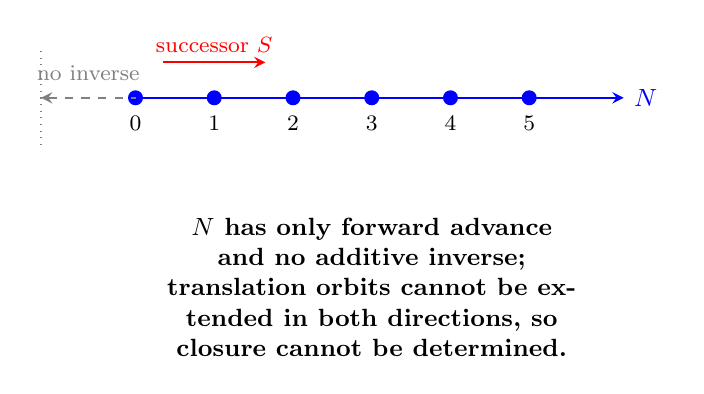
\begin{tikzpicture}[scale=1.0,>=stealth]
        \draw[->, thick, blue] (0,0) -- (6.2,0) node[right, font=\small] {$\mathbb{N}$};
        \foreach \x in {0,1,2,...,5} {
            \filldraw[blue] (\x,0) circle (2.5pt);
            \node[below=3pt, font=\footnotesize] at (\x,0) {$\x$};
        }
        \draw[->, red, thick] (0.35,0.45) -- (1.65,0.45)
            node[midway, above, font=\footnotesize] {successor $S$};
        \draw[<-, gray, dashed, thick] (-1.2,0) -- (0,0);
        \node[gray, font=\footnotesize, above] at (-0.6,0.1) {no inverse};
        \draw[gray, dotted] (-1.2,-0.6) -- (-1.2,0.6);
        \node[font=\small\bfseries, text width=7.5cm, align=center, below=1.4cm] at (3,0)
            {$\mathbb{N}$ has only forward advance and no additive inverse;\\ translation orbits cannot be extended in both directions, so closure cannot be determined.};
    \end{tikzpicture}
    \caption{The ray structure of the natural numbers $\mathbb{N}$. The successor map $S$ provides only one-directional advance, with no inverse map. Translation orbits cannot be traced backwards, and closure determination is not closed in $\mathbb{N}$ (Proposition \ref{prop:natural_no_inverse}).}
    \label{fig:natural_ray}
\end{figure}
\begin{corollary}[The relationship between the natural numbers and period determination]\label{cor:natural_period}
The natural numbers have no centre of symmetry and no directional duality, and do not themselves form a group; hence they do not directly provide an algebraic tool for period determination. In the spectrum of periodic mathematics, $\mathbb{N}$ provides only the function of counting---the numbering of `the $k$-th element' in a periodic sequence. The determination of discrete translation periods requires at least the group structure of $\mathbb{Z}$ (deduced from Proposition \ref{prop:natural_no_inverse}).
\end{corollary}

\begin{proof}
By Proposition \ref{prop:natural_no_inverse}, subtraction, division and root extraction are all non-closed in $\mathbb{N}$, so there is no additive inverse and no multiplicative inverse. Without inverses there is no `reverse' operation, and therefore neither a centre of symmetry (symmetry requires $x \mapsto -x$ or $x \mapsto x^{-1}$ to be defined) nor a directional duality (a direction requires forward and reverse to occur in pairs). The determination of discrete translation periods requires that orbits can be extended in both directions and their closure tested, which requires at least additive inverses, that is, the group structure of $\mathbb{Z}$.
\end{proof}

\subsection{\texorpdfstring{Function-theoretic features: solvability of the translation equation and the absence of a group with periodic orbits}{Function-theoretic features: solvability of the translation equation and the absence of a group with periodic orbits}}

\begin{proposition}[Solution of the translation equation on the natural numbers]\label{prop:translation_equation_N}
Let $f:\mathbb{N}\to Y$, $a\in\mathbb{N}$, $a\ne0$. If
\[
f(x+a)=f(x),\qquad \forall x\in\mathbb{N},
\]
then $f$ is constant on each residue class modulo $a$; but the period set
\[
\operatorname{Group}_{\mathrm{period},\mathbb{N}}(f)=\{a\in\mathbb{N}: f(x+a)=f(x),\ \forall x\in\mathbb{N}\}
\]
is in general \textbf{not a subgroup}, because no additive inverse exists in $\mathbb{N}$: $a\in\operatorname{Group}_{\mathrm{period},\mathbb{N}}(f)$ does not imply that $-a$ exists.
\end{proposition}

\begin{proof}
Iterating $f(x+a)=f(x)$ repeatedly gives $f(x+na)=f(x)$ for every $n\in\mathbb{N}$, so $f$ is constant on the residue classes modulo $a$. But closure of the period set requires inverses: if $a,b\in\operatorname{Group}_{\mathrm{period},\mathbb{N}}(f)$, then $a+b\in\operatorname{Group}_{\mathrm{period},\mathbb{N}}(f)$ (since $f(x+a+b)=f(x+a)=f(x)$), but $a-b$ need not lie in $\mathbb{N}$, so the subgroup criterion is not satisfied.
\end{proof}

\begin{proposition}[Failure of the antiperiod equation on the natural numbers]\label{prop:antiperiod_N}
Let $f:\mathbb{N}\to Y$, $a\in\mathbb{N}$, $a\ne0$. If
\[
f(x+a)=-f(x),\qquad \forall x\in\mathbb{N},
\]
then iteration gives $f(x+2a)=f(x)$, so $2a\in\operatorname{Group}_{\mathrm{period},\mathbb{N}}(f)$. But the equation itself cannot be extended backwards: $f(x-a)$ is undefined when $x<a$.
\end{proposition}

\begin{proof}
From $f(x+a)=-f(x)$ we obtain $f(x+2a)=f(x)$. Backward extension requires $x-a\in\mathbb{N}$, that is, $x\ge a$, so it fails at $x<a$.
\end{proof}

\begin{remark}[Status of the scaling and rotation equations on the natural numbers]\label{rem:scaling_rotation_N}
The scaling equation $f(qx)=f(x)$ is meaningful on $\mathbb{N}$ only when $q$ is an integer and $q$ divides every relevant $x$, and $q^{-1}$ does not exist, so two-directional iteration is impossible. The rotation equation $f(e^{i\theta}z)=f(z)$ has no algebraic carrier at all in $\mathbb{N}$, because $e^{i\theta}$ does not belong to $\mathbb{N}$. Thus the natural numbers carry only the most primitive form of the translation equation, and the group with periodic orbits is not closed.
\end{remark}

\section{\texorpdfstring{The integers $\mathbb{Z}$: the basis for determining discrete translation periods}{The integers Z: the basis for determining discrete translation periods}}

\subsection{\texorpdfstring{Determination requirement}{Determination requirement}}

Given the translation orbit
\[
\mathcal{O}(x_0; T) = \{x_0 + nT \mid n \in \mathbb{Z}\},
\]
determining whether it is regular and whether it can close presupposes that the orbit must be extendable in both directions. If there is only forward advance, it can never `return to the starting point', and closure determination is logically impossible.

\subsection{\texorpdfstring{Algebraic requirement}{Algebraic requirement}}

Additive inverses, that is, subtraction. This is the minimal algebraic closure that makes translation a group action.

\subsection{\texorpdfstring{Construction of the integers}{Construction of the integers}}

\begin{definition}[Construction of the integers]\label{def:integer_construction}
Define an equivalence relation on $\mathbb{N} \times \mathbb{N}$ by
\[
(a,b) \sim (c,d) \iff a + d = b + c.
\]
The set of integers is $\mathbb{Z} := (\mathbb{N} \times \mathbb{N}) / \sim$. The equivalence class $[(a,b)]$ corresponds to the intuitive `$a - b$'.

Definitions of the operations:
\begin{itemize}
    \item Addition: $[(a,b)] + [(c,d)] := [(a+c, b+d)]$.
    \item Zero element: $0_{\mathbb{Z}} := [(0,0)]$.
    \item Additive inverse: $-[(a,b)] := [(b,a)]$.
    \item Multiplication: $[(a,b)] \times [(c,d)] := [(ac+bd, ad+bc)]$.
\end{itemize}
\end{definition}

\begin{proposition}[The integer operations are well defined]\label{prop:integer_well_defined}
The above definitions of addition and multiplication do not depend on the choice of representative, and $(\mathbb{Z},+,\times)$ forms a commutative ring.
\end{proposition}

\begin{proof}
Let $(a,b) \sim (a',b')$ and $(c,d) \sim (c',d')$, that is,
\[
a+b' = b+a', \qquad c+d' = d+c'. \tag{*}
\]
Well-definedness of addition: we must prove $(a+c, b+d) \sim (a'+c', b'+d')$, that is,
\[
(a+c)+(b'+d') = (b+d)+(a'+c').
\]
Adding the two equations in $(*)$ and using associativity and commutativity gives:
\[
(a+c)+(b'+d') = (a+b')+(c+d') = (b+a')+(d+c') = (b+d)+(a'+c').
\]
Well-definedness of multiplication: we must prove $(ac+bd, ad+bc) \sim (a'c'+b'd', a'd'+b'c')$, that is,
\[
ac + bd + a'd' + b'c' = ad + bc + a'c' + b'd'. \tag{**}
\]
From $(*)$ we obtain $a + b' = b + a'$; multiplying the two sides by $c$ and by $d$ respectively gives
\[
ac + b'c = bc + a'c, \qquad bd + a'd = ad + b'd.
\]
Hence
\[
ac + bd + a'd + b'c = (ac + b'c) + (bd + a'd) = (bc + a'c) + (ad + b'd) = ad + bc + a'c + b'd,
\]
that is, $(ac+bd, ad+bc) \sim (a'c+b'd, a'd+b'c)$, so multiplication is well defined in the first factor. Similarly, from $(c,d) \sim (c',d')$ we obtain well-definedness of multiplication in the second factor. Composing the two substitutions gives $(ac+bd, ad+bc) \sim (a'c'+b'd', a'd'+b'c')$, so multiplication is well defined.

Ring axioms: the associativity and commutativity of addition, the zero element $[(0,0)]$ and the inverse $-[(a,b)] = [(b,a)]$ are inherited directly from the corresponding properties of the natural numbers through representatives; the associativity of multiplication and the distributive law follow likewise, verified by expanding term by term through representatives, and all of them reduce to the laws of operation for the natural numbers.
\end{proof}

\subsection{\texorpdfstring{Operational duality and directional structure in the integers}{Operational duality and directional structure in the integers}}

\begin{proposition}[Operational duality in the integers]\label{prop:integer_operation_duality}
In $\mathbb{Z}$:
\begin{enumerate}[label=(\roman*)]
    \item \textbf{Addition and subtraction} form a complete duality: $a + x = b \iff x = b - a$. Forward direction: $x \mapsto x + k$ (translation to the right); reverse direction: $x \mapsto x - k$ (translation to the left).
    \item \textbf{Multiplication} is closed, but \textbf{division} is still incomplete: when $a \neq 0$, the equation $a \times x = b$ has an integer solution if and only if $a \mid b$; when $a = 0$, it has a solution if and only if $b = 0$ (in which case every $x$ is a solution).
    \item \textbf{Powers} are closed (integer base, natural-number exponent), but \textbf{roots} are still incomplete.
\end{enumerate}
\end{proposition}

\begin{proof}
(i) If $x = b - a = b + (-a)$, then $a + x = a + b + (-a) = b$; conversely, if $a + x = b$, adding $-a$ to both sides gives $x = b + (-a) = b - a$. Hence $a + x = b \iff x = b - a$, and addition and subtraction form a complete duality. The directional duality is given by $x \mapsto x + k$ and its inverse map $x \mapsto x - k$: $(x+k)-k = x = (x-k)+k$.
(ii) Let $a \neq 0$. If $a \mid b$, then there exists $c \in \mathbb{Z}$ with $b = ac$, and $x = c$ is a solution; conversely, if $ax = b$ has an integer solution, then $a \mid b$. Let $a = 0$; the equation becomes $0 = b$: when $b = 0$ every $x$ is a solution, and when $b \neq 0$ there is no solution. In summary, division is closed only in the case of exact divisibility, and is not closed in general.
(iii) For an integer $b$ and a non-negative integer $n$, $b^n$ is obtained by multiplying $b$ by itself repeatedly and is still an integer, so powers are closed. For root extraction: the equation $x^e = b$ has an integer solution if and only if $b$ is the $e$-th power of some integer (and when $e$ is even one requires $b \geq 0$); it is not closed in general, for example $x^2 = 2$ has no integer solution.
\end{proof}

\begin{proposition}[Symmetry, directionality and periodicity of the integers]\label{prop:integer_symmetry_direction_period}
The operational structure on the integers gives rise to the following symmetries and periodicities:
\begin{enumerate}[label=(\roman*)]
    \item \textbf{Centre of symmetry}: $0$ (the additive identity).
    \item \textbf{Type of symmetry}: additive reflection symmetry. $\sigma_{0,+}(x) = -x$ is an involutive automorphism with fixed point $0$, generating the group $C_2$.
    \item \textbf{Directional structure}: the translation direction. Direction group $\langle 1 \rangle = \mathbb{Z}$. Forward: $x \mapsto x + 1$; reverse: $x \mapsto x - 1$.
    \item \textbf{Type of period}: translation quasi-period. The orbit $\{a_0 + k \mid k \in \mathbb{Z}\}$ extends isometrically on $\mathbb{Z}$. The translation-invariant functions on this orbit are the constant functions.
\end{enumerate}
\end{proposition}

\begin{proof}
(i) $0 + x = x$ holds for all $x \in \mathbb{Z}$, and for every $x$ there exists a unique $-x$ with $x + (-x) = 0$.
(ii) $\sigma_{0,+}(\sigma_{0,+}(x)) = -(-x) = x$, so it is an involution. The fixed-point condition is $-x = x \iff 2x = 0 \iff x = 0$ (in a torsion-free additive group).
(iii) Every integer can be written uniquely as $n \cdot 1$ ($n \in \mathbb{Z}$), with the forward direction corresponding to $n>0$ and the reverse direction to $n<0$.
(iv) For every $k \in \mathbb{Z}$, $T_k(x) = x + k$ satisfies $T_k \circ T_{-k} = \text{id}$. The isometry of the orbit is guaranteed by $|(x+k) - x| = |k|$. The translation group acts transitively on $\mathbb{Z}$, so its invariants must be constant functions $P(x) = \text{const}$.
\end{proof}

\subsection{\texorpdfstring{Function-theoretic features: invertibilisation of the translation equation and the group with periodic orbits}{Function-theoretic features: invertibilisation of the translation equation and the group with periodic orbits}}

\begin{theorem}[The group with periodic orbits of the translation equation on the integers]\label{thm:translation_equation_Z}
Let $f:\mathbb{Z}\to Y$, $a\in\mathbb{Z}$, $a\ne0$. If
\[
f(x+a)=f(x),\qquad \forall x\in\mathbb{Z},
\]
then the group with periodic orbits
\[
\operatorname{Group}_{\mathrm{period},\mathbb{Z}}(f)=\{T\in\mathbb{Z}: f(x+T)=f(x),\ \forall x\in\mathbb{Z}\}
\]
is a subgroup of $\mathbb{Z}$, and $a\mathbb{Z}\le\operatorname{Group}_{\mathrm{period},\mathbb{Z}}(f)$.
\end{theorem}

\begin{proof}
Iterating $f(x+a)=f(x)$ in both directions gives $f(x+na)=f(x)$ for every $n\in\mathbb{Z}$, so $a\mathbb{Z}\le\operatorname{Group}_{\mathrm{period},\mathbb{Z}}(f)$. The period set is closed under addition and under taking inverses ($T\in\operatorname{Group}_{\mathrm{period},\mathbb{Z}}(f)\Rightarrow -T\in\operatorname{Group}_{\mathrm{period},\mathbb{Z}}(f)$ is guaranteed by two-directional extension), hence it is a subgroup.
\end{proof}

\begin{corollary}[Period doubling for the antiperiod equation]\label{cor:antiperiod_Z}
If $f(x+a)=-f(x)$ holds for all $x\in\mathbb{Z}$, then $f(x+2a)=f(x)$, that is, $2a\in\operatorname{Group}_{\mathrm{period},\mathbb{Z}}(f)$, and $2a\mathbb{Z}\le\operatorname{Group}_{\mathrm{period},\mathbb{Z}}(f)$.
\end{corollary}

\begin{proof}
From $f(x+a)=-f(x)$ we obtain $f(x+2a)=f(x)$. Here $f(x-a)$ is defined for all $x\in\mathbb{Z}$, and the group with periodic orbits is complete.
\end{proof}

\begin{figure}[htbp]
    \centering
    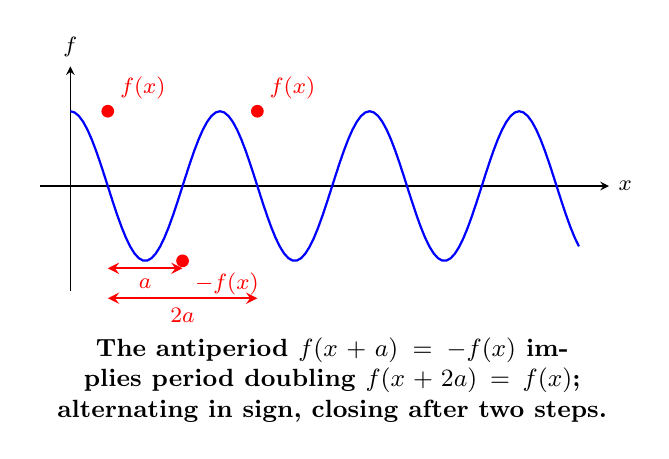
\begin{tikzpicture}[scale=0.95,>=stealth]
        \draw[->] (-0.4,0) -- (7.2,0) node[right, font=\footnotesize] {$x$};
        \draw[->] (0,-1.4) -- (0,1.6) node[above, font=\footnotesize] {$f$};
        \draw[thick, blue, domain=0:6.8, samples=120]
            plot (\x, {cos(180*\x)});
        \draw[<->, red, thick] (0.5,-1.1) -- (1.5,-1.1)
            node[midway, below, font=\footnotesize] {$a$};
        \draw[<->, red, thick] (0.5,-1.5) -- (2.5,-1.5)
            node[midway, below, font=\footnotesize] {$2a$};
        \filldraw[red] (0.5,1) circle (2.2pt);
        \filldraw[red] (1.5,-1) circle (2.2pt);
        \filldraw[red] (2.5,1) circle (2.2pt);
        \node[red, font=\footnotesize, above right=1pt] at (0.5,1) {$f(x)$};
        \node[red, font=\footnotesize, below right=1pt] at (1.5,-1) {$-f(x)$};
        \node[red, font=\footnotesize, above right=1pt] at (2.5,1) {$f(x)$};
        \node[font=\small\bfseries, text width=7.5cm, align=center, below=1.8cm] at (3.5,0)
            {The antiperiod $f(x+a)=-f(x)$ implies period doubling $f(x+2a)=f(x)$;\\ alternating in sign, closing after two steps.};
    \end{tikzpicture}
    \caption{The geometric picture of the antiperiod equation $f(x+a)=-f(x)$. The function has opposite signs on two adjacent $a$-intervals, and after two steps returns to its initial value---the period doubles to $2a$ (Corollary \ref{cor:antiperiod_Z}). This is the simplest non-trivial period-doubling structure.}
    \label{fig:antiperiod_doubling}
\end{figure}

\begin{remark}[The integers make the translation equation invertible]\label{rem:integer_makes_translation_invertible}
In the natural numbers the translation equation can be iterated in one direction only, and the period set is not closed; in the integers additive inverses exist, the translation equation can be iterated in both directions, and the period set becomes a subgroup. This is the first instance of number-system extension making a function equation pass from `non-invertible' to `invertible'.
\end{remark}

\begin{figure}[htbp]
    \centering
    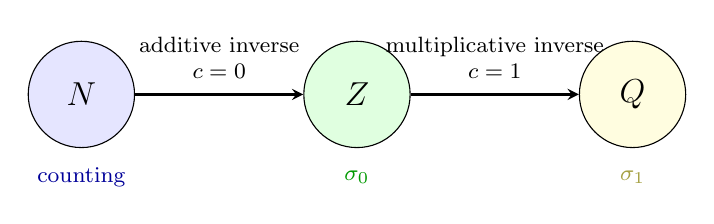
\begin{tikzpicture}[>=stealth,
        nsbox/.style={draw, circle, minimum size=1.35cm, inner sep=0pt,
                      font=\large\bfseries},
        arrow/.style={->, thick, >=stealth},
        lbl/.style={font=\footnotesize, midway, above=2pt, align=center},
        sublbl/.style={font=\footnotesize, align=center}]

        \node[nsbox, fill=blue!10]   (N) at (0,0)    {$\mathbb{N}$};
        \node[nsbox, fill=green!12]  (Z) at (3.5,0)  {$\mathbb{Z}$};
        \node[nsbox, fill=yellow!12] (Q) at (7.0,0)  {$\mathbb{Q}$};

        \draw[arrow] (N) -- (Z) node[lbl] {additive inverse\\ $c=0$};
        \draw[arrow] (Z) -- (Q) node[lbl] {multiplicative inverse\\ $c=1$};

        \node[sublbl, blue!60!black]   at (0,   -1.05) {counting};
        \node[sublbl, green!60!black]  at (3.5, -1.05) {$\sigma_0$};
        \node[sublbl, yellow!60!black] at (7.0, -1.05) {$\sigma_1$};

    \end{tikzpicture}
    \caption{The level-by-level emergence of the centres of symmetry $0$, $1$ in number-system extension (local diagram of Section \ref{prop:integer_symmetry_direction_period}). $\mathbb{N}\to\mathbb{Z}$ introduces additive inverses (centre of symmetry $0$); $\mathbb{Z}\to\mathbb{Q}$ introduces multiplicative inverses (centre of symmetry $1$). The subsequent extensions $\mathbb{R}$, $\mathbb{C}$, $\mathbb{H}$ (introducing completeness, the imaginary unit $i$ and non-commutative multiplication respectively) are shown in the chapter summary diagram \ref{fig:number_extension}.}
    \label{fig:symmetry_centre_emergence}
\end{figure}
\subsection{\texorpdfstring{Criterion theorem}{Criterion theorem}}

\begin{lemma}[Order of an element in a finite cyclic group]\label{lem:order_cyclic_subgroup_ch2}
Let $m \ge 1$ and $T \in \mathbb{Z}$. In the quotient group $\mathbb{Z}/m\mathbb{Z}$, the cyclic subgroup $\langle [T] \rangle$ generated by the element $[T]$ has order $m/\gcd(T,m)$. In particular, $\gcd(T,m) = 1$ if and only if $[T]$ generates the whole of $\mathbb{Z}/m\mathbb{Z}$.
\end{lemma}

\begin{proof}
Let $d = \gcd(T,m)$. The order of $[T]$ is the least positive integer $n$ for which $nT \equiv 0 \pmod{m}$. The condition $m \mid nT$ is equivalent to $\frac{m}{d} \mid n \cdot \frac{T}{d}$. Since $\gcd\!\left(\frac{m}{d}, \frac{T}{d}\right) = 1$, the coprimality property gives $\frac{m}{d} \mid n$, and the least positive integer solution is $n = \frac{m}{d} = \frac{m}{\gcd(T,m)}$. When $\gcd(T,m) = 1$ we have $d = 1$, so $[T]$ has order $m = |\mathbb{Z}/m\mathbb{Z}|$ and hence $[T]$ generates the whole group; conversely, if $[T]$ generates the whole group, then its order is $m$, that is, $m = m/d$, giving $d = 1$.
\end{proof}

\begin{theorem}[Criterion for integer translation periods]\label{thm:integer_translation_criterion}
Let $x_0 \in \mathbb{Z}$ and let the translation step be $T \in \mathbb{Z}$. Then:
\begin{enumerate}[label=(\roman*)]
    \item If $T = 0$, the orbit $\mathcal{O}(x_0; T)$ degenerates to the single point $\{x_0\}$, with period $1$ (the trivial period).
    \item If $T \neq 0$, the orbit $\mathcal{O}(x_0; T)$ is a two-directionally infinite isometric sequence of points, non-closed but regular. In any finite quotient $\mathbb{Z}/m\mathbb{Z}$ (that is, $C_m$), the orbit necessarily closes, with period exactly $m/\gcd(T,m)$; in particular, the orbit degenerates to a single point if and only if $T \equiv 0 \pmod{m}$.
\end{enumerate}
\end{theorem}

\begin{proof}
(i) $x_0 + n\cdot 0 = x_0$ for all $n$, so the orbit contains only one point.
(ii) If $T \neq 0$, then $|(x_0+nT) - x_0| = |nT|$ increases without bound as $|n|$ grows, so the orbit does not close in $\mathbb{Z}$. In the quotient group $\mathbb{Z}/m\mathbb{Z}$ the orbit is the coset $[x_0] + \langle [T] \rangle$; by Lemma \ref{lem:order_cyclic_subgroup_ch2}, $\mathrm{ord}([T]) = m/\gcd(T,m)$ is finite, so the orbit closes with period $m/\gcd(T,m)$. In particular, the orbit degenerates to a single point if and only if $[T] = [0]$, that is, $T \equiv 0 \pmod{m}$.
\end{proof}

\begin{corollary}[Integers and discrete translation periods]\label{cor:integer_discrete_translation}
$\mathbb{Z}$ is the minimal group structure in which discrete translation periods can be determined (deduced from Theorem \ref{thm:integer_translation_criterion}). Its determining power is reflected in:
\begin{enumerate}[label=(\roman*)]
    \item orbits can be extended in both directions, and this traceability makes closure determination possible;
    \item the quotient structure of the finite cyclic group $C_m \cong \mathbb{Z}/m\mathbb{Z}$ gives finite translation periods an exact algebraic characterisation.
\end{enumerate}
\end{corollary}

\begin{proof}
(i) The argument for the case $T \neq 0$ in Theorem \ref{thm:integer_translation_criterion} relies on additive inverses in $\mathbb{Z}$: the existence of the negative translation $x \mapsto x - T$ makes orbits traceable, so that closure determination becomes possible.
(ii) By Lemma \ref{lem:order_cyclic_subgroup_ch2}, the order (period) of an element of $C_m \cong \mathbb{Z}/m\mathbb{Z}$ can be computed exactly as $m/\gcd(T,m)$, so finite translation periods acquire an algebraic characterisation.
\end{proof}

\begin{figure}[htbp]
\centering
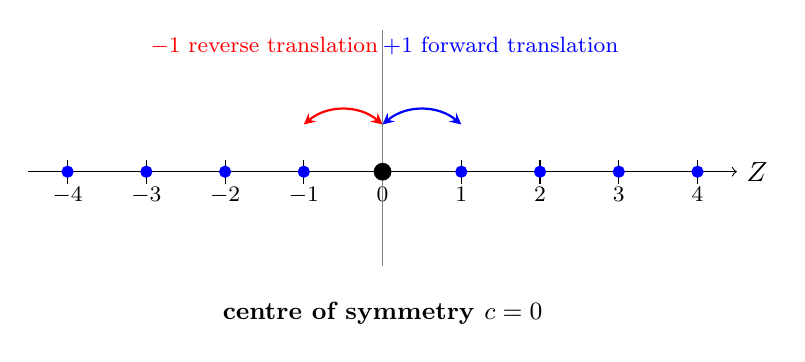
\begin{tikzpicture}[scale=1.0]
    \draw[->] (-4.5,0) -- (4.5,0) node[right] {$\mathbb{Z}$};
    \foreach \i in {-4,...,4} {
        \draw (\i, 0.15) -- (\i, -0.15);
        \node[below=2pt, font=\footnotesize] at (\i,0) {$\i$};
        \filldraw[blue] (\i, 0) circle (2pt);
    }
    \draw[<->, blue, thick, >=stealth] (0, 0.6) to[bend left=40] (1, 0.6);
    \node[blue, font=\footnotesize] at (1.5, 1.6) {$+1$ forward translation};
    \draw[<->, red, thick, >=stealth] (0, 0.6) to[bend right=40] (-1, 0.6);
    \node[red, font=\footnotesize] at (-1.5, 1.6) {$-1$ reverse translation};
    \draw[gray, thin] (0, -1.2) -- (0, 1.8);
    \node[font=\small\bfseries] at (0, -1.8) {centre of symmetry $c=0$};
    \filldraw[black] (0,0) circle (3pt);
\end{tikzpicture}
\caption{The translation direction structure of the integers $\mathbb{Z}$: with $0$ as centre of symmetry, $+1$ and $-1$ form a forward--reverse directional duality. The orbit extends isometrically on the integer axis.}
\label{fig:integer_direction}
\end{figure}
\section{\texorpdfstring{The rationals $\mathbb{Q}$: the basis for determining finite rotation periods}{The rationals Q: the basis for determining finite rotation periods}}

\subsection{\texorpdfstring{Determination requirement}{Determination requirement}}

When does the rotation orbit
\[
\mathcal{O}(z_0; \theta) = \{z_0 e^{in\theta} \mid n\in\mathbb{Z}\}
\]
close? The criterion is
\[
\frac{\theta}{2\pi} \in \mathbb{Q}.
\]
But the very concept of `commensurability' itself requires the rational numbers. Without $\mathbb{Q}$ we could not even express that `the rotation angle is commensurable with one third of the circumference'.

\subsection{\texorpdfstring{Algebraic requirement}{Algebraic requirement}}

Multiplicative inverses, that is, division. This is the minimal algebraic closure that makes proportional relations exactly expressible.

\subsection{\texorpdfstring{Construction of the rational numbers}{Construction of the rational numbers}}

\begin{definition}[Construction of the rational numbers]\label{def:rational_construction}
Define an equivalence relation on $\mathbb{Z} \times \mathbb{Z}^{\times}$ (where $\mathbb{Z}^{\times} = \mathbb{Z} \setminus \{0\}$) by
\[
(a,b) \approx (c,d) \iff a \times d = b \times c.
\]
The set of rational numbers is $\mathbb{Q} := (\mathbb{Z} \times \mathbb{Z}^{\times}) / \approx$. Equivalence classes are written $\frac{a}{b}$ or $a/b$.

Definitions of the operations:
\begin{itemize}
    \item Addition: $\frac{a}{b} + \frac{c}{d} := \frac{ad+bc}{bd}$.
    \item Multiplication: $\frac{a}{b} \times \frac{c}{d} := \frac{ac}{bd}$.
    \item Additive zero element: $\frac{0}{1}$.
    \item Multiplicative identity: $\frac{1}{1}$.
    \item Additive inverse: $-\frac{a}{b} := \frac{-a}{b}$.
    \item Multiplicative inverse: $(\frac{a}{b})^{-1} := \frac{b}{a}$ ($a \neq 0$).
\end{itemize}
\end{definition}

\begin{proposition}[The rational numbers form a field]\label{prop:rational_field}
$(\mathbb{Q},+,\times)$ forms a field, that is, it is simultaneously an additive abelian group and a multiplicative abelian group (apart from the zero element), and multiplication satisfies the distributive law over addition.
\end{proposition}

\begin{proof}
The additive group structure is inherited from the fraction construction of $\mathbb{Z}$. The associativity and commutativity of multiplication are verified directly from integer multiplication. Existence of multiplicative inverses: for any $\frac{a}{b} \neq 0$ (that is, $a \neq 0$), the inverse is $\frac{b}{a} \in \mathbb{Q}$. The distributive law is verified by computation over a common denominator.
\end{proof}

\subsection{\texorpdfstring{The centre of symmetry $1$ and the proportional direction}{The centre of symmetry 1 and the proportional direction}}

\begin{definition}[The taking-the-inverse involution $\sigma_1$]\label{def:rational_involution}
On the multiplicative group $\mathbb{Q}^{\times} = \mathbb{Q} \setminus \{0\}$, define the map
\[
\sigma_1: \mathbb{Q}^{\times} \to \mathbb{Q}^{\times}, \quad \sigma_1(x) = x^{-1} = \frac{1}{x}.
\]
The map $\sigma_1$ is called the involution about the centre of symmetry $1$.
\end{definition}

\begin{proposition}[Basic properties of the involution $\sigma_1$]\label{prop:rational_involution_properties}
\begin{enumerate}[label=(\roman*)]
    \item $\sigma_1$ is an involution: $\sigma_1 \circ \sigma_1 = \text{id}_{\mathbb{Q}^{\times}}$.
    \item The fixed-point set of $\sigma_1$ is $\{1, -1\}$.
    \item $\sigma_1$ is an automorphism of the multiplicative group $(\mathbb{Q}^{\times}, \times)$: $\sigma_1(x \times y) = \sigma_1(x) \times \sigma_1(y)$.
    \item $\sigma_1$ interchanges the operation of `enlargement' (multiplication by $q>1$) with the operation of `shrinkage' (division by $q$).
\end{enumerate}
\end{proposition}

\begin{proof}
(i) $\sigma_1(\sigma_1(x)) = 1/(1/x) = x$.
(ii) $\sigma_1(x) = x \iff 1/x = x \iff x^2 = 1 \iff x = 1$ or $x = -1$.
(iii) $\sigma_1(xy) = 1/(xy) = (1/x)(1/y) = \sigma_1(x) \sigma_1(y)$.
(iv) Let $T_q(x) = qx$ ($q>1$, enlargement); then $\sigma_1 \circ T_q \circ \sigma_1(x) = \sigma_1(q \cdot x^{-1}) = x/q$, that is, the shrinking operation.
\end{proof}

\begin{proposition}[Directional structure and period types of the rational numbers]\label{prop:rational_direction_period}
Building on the symmetries of the integers, the rational numbers acquire the following additional structure:
\begin{enumerate}[label=(\roman*)]
    \item \textbf{New centre of symmetry}: $1$ (the multiplicative identity).
    \item \textbf{New type of symmetry}: multiplicative inversion symmetry. $\sigma_1(x) = x^{-1}$ is an involutive automorphism of the multiplicative group $\mathbb{Q}^{\times}$, with fixed points $\pm 1$.
    \item \textbf{New directional structure}: the proportional direction. Direction group $\langle q \rangle = \{q^k \mid k \in \mathbb{Z}\} \cong \mathbb{Z}$ ($q > 0, q \neq 1$). Forward: $x \mapsto q \times x$; reverse: $x \mapsto x / q$.
    \item \textbf{New type of period}: proportional quasi-period. Via the logarithmic homomorphism, the orbit $\{a_0 q^k \mid k \in \mathbb{Z}\}$ is equivalent to a translation quasi-period in the logarithmic domain.
\end{enumerate}
\end{proposition}

\begin{proof}
(i)--(ii) The properties of the centre of symmetry $1$ and of the multiplicative inversion symmetry $\sigma_1$ have already been established by Definition \ref{def:rational_involution} and Proposition \ref{prop:rational_involution_properties}.
(iii) For $q > 0, q \neq 1$, the map $k \mapsto q^k$ gives a group isomorphism $\mathbb{Z} \to \langle q \rangle$: $q^{k_1 + k_2} = q^{k_1} q^{k_2}$ and $q^0 = 1$, and moreover $q^{k_1} = q^{k_2}$ if and only if $k_1 = k_2$ (for $q \neq 1$ the function $q^k$ is strictly monotone), so $\langle q \rangle \cong \mathbb{Z}$. The forward map $x \mapsto qx$ corresponds to $k \mapsto k+1$, and the reverse map $x \mapsto x/q$ corresponds to $k \mapsto k-1$.
(iv) Under the logarithmic map $\ln$, the orbit $\{a_0 q^k \mid k \in \mathbb{Z}\}$ becomes $\{\ln a_0 + k \ln q \mid k \in \mathbb{Z}\}$, an isometric translation orbit on $\mathbb{R}$ with step $\ln q$ (see Proposition \ref{prop:rational_momentum} and Figure \ref{fig:rational_direction}); it is therefore the dual, in the proportional direction, of the translation quasi-period---the proportional quasi-period.
\end{proof}

\subsection{\texorpdfstring{Function-theoretic features: the scaling equation and commensurability}{Function-theoretic features: the scaling equation and commensurability}}

\begin{theorem}[The group with periodic orbits of the scaling equation on the rationals]\label{thm:scaling_equation_Q}
Let $f:\mathbb{Q}^+\to Y$, $q\in\mathbb{Q}^+$, $q\ne1$. If
\[
f(qx)=f(x),\qquad \forall x\in\mathbb{Q}^+,
\]
then the group with periodic orbits
\[
\operatorname{Group}_{\mathrm{period},\mathbb{Q}^+}(f)=\{r\in\mathbb{Q}^+: f(rx)=f(x),\ \forall x\in\mathbb{Q}^+\}
\]
is a subgroup of $\mathbb{Q}^+$, and $\langle q\rangle=\{q^n:n\in\mathbb{Z}\}\le\operatorname{Group}_{\mathrm{period},\mathbb{Q}^+}(f)$.
\end{theorem}

\begin{proof}
Iterating $f(qx)=f(x)$ in both directions gives $f(q^n x)=f(x)$ for every $n\in\mathbb{Z}$ (since $q^{-1}$ exists in $\mathbb{Q}^+$), so $\langle q\rangle\le\operatorname{Group}_{\mathrm{period},\mathbb{Q}^+}(f)$. The period set is closed under multiplication and under taking inverses, hence it is a subgroup.
\end{proof}

\begin{theorem}[The rationals and the commensurability criterion for the rotation equation]\label{thm:rotation_equation_Q}
Let $\theta\in\mathbb{R}$ and $f:\mathbb{C}^\times\to Y$. The rotation equation
\[
f(e^{i\theta}z)=f(z),\qquad \forall z\in\mathbb{C}^\times
\]
has a non-trivial periodic solution whenever $\theta/(2\pi)\in\mathbb{Q}$; alongside this, the group with periodic orbits $\langle e^{i\theta}\rangle\le\mathbb{C}^\times$ generated by the rotation is finite if and only if $\theta/(2\pi)\in\mathbb{Q}$. This criterion itself relies on the fractional representation $p/q$ of the rational numbers $\mathbb{Q}$. Hence $\mathbb{Q}$ is the minimal algebraic structure for expressing `commensurability', but the \textbf{algebraic realisation} of the rotation equation (the construction of $e^{i\theta}$) still requires $\mathbb{C}$.
\end{theorem}

\begin{proof}
First assertion (the sufficient direction): if $\theta/(2\pi)=p/q\in\mathbb{Q}$ in lowest terms, then $e^{i\theta}$ is a $q$-th root of unity, and $f(e^{i\theta}z)=f(z)$ has a non-trivial solution---take $f(z)=z^{q}$; then $f(e^{i\theta}z)=(e^{i\theta}z)^{q}=e^{2\pi ip}z^{q}=f(z)$, and $f$ is not constant.

Second assertion (the group with periodic orbits): if $\theta/(2\pi)=p/q\in\mathbb{Q}$ in lowest terms, then $e^{i\theta}$ has order $q$ and $\langle e^{i\theta}\rangle$ is finite; conversely, if $\theta/(2\pi)\notin\mathbb{Q}$, then $e^{in\theta}=1$ would require $\theta/(2\pi)=k/n\in\mathbb{Q}$, so $e^{i\theta}$ has infinite order and $\langle e^{i\theta}\rangle$ is infinite.

Expressing the criterion $\theta/(2\pi)\in\mathbb{Q}$ requires $\mathbb{Q}$, but the algebraisation of $e^{i\theta}$ itself requires $i$ in $\mathbb{C}$.
\end{proof}

\begin{remark}[The first assertion of Theorem \ref{thm:rotation_equation_Q} does not reverse]\label{rem:rotation_equation_Q_converse}
The first assertion of Theorem \ref{thm:rotation_equation_Q} is one-directional: $\theta/(2\pi)\in\mathbb{Q}$ guarantees a non-trivial periodic solution, but the existence of a solution does not imply that $\theta/(2\pi)\in\mathbb{Q}$. The existence of solutions is determined by the level sets of $f$ alone and is independent of the order of $e^{i\theta}$: the functions satisfying the rotation equation pointwise are exactly those constant on the $\langle e^{i\theta}\rangle$-orbits, a class that varies with $\theta$, yet is non-empty for every $\theta$. The reverse direction requires an additional restriction on $f$; for instance, if $f$ is continuous and non-constant on some circle $|z|=r$, then $\theta/(2\pi)\notin\mathbb{Q}$ forces every solution to be trivial, because $e^{i\theta}$ is dense on that circle and continuity then forces $f$ to be constant on the whole circle. The second assertion (finiteness of the group with periodic orbits), by contrast, remains an equivalence once it is stated in terms of the group with periodic orbits $\langle e^{i\theta}\rangle$.
\end{remark}

\begin{example}[A pointwise periodic solution does not imply finite order]\label{ex:rotation_equation_module}
Take $f(z)=|z|$. Then for every $\theta\in\mathbb{R}$ and every $z\in\mathbb{C}^\times$,
\[
f(e^{i\theta}z)=|e^{i\theta}z|=|z|=f(z),
\]
so every $\theta$ admits a pointwise periodic solution; in particular, when $\theta/(2\pi)\notin\mathbb{Q}$ (for example $\theta=1$) the group with periodic orbits $\langle e^{i\theta}\rangle$ of the rotation is still infinite. Hence `admitting a pointwise periodic solution' is strictly weaker than `the rotation has finite order', and the first assertion of Theorem \ref{thm:rotation_equation_Q} cannot be written as an `if and only if'.
\end{example}

\begin{remark}[The rationals make the scaling equation invertible]\label{rem:rational_makes_scaling_invertible}
In the integers the scaling equation $f(qx)=f(x)$ is meaningful only when $q$ divides every relevant $x$, and $q^{-1}$ does not exist. In the rationals multiplicative inverses exist, the scaling equation can be iterated in both directions, and the group with periodic orbits $\langle q\rangle$ becomes a subgroup. This is the second instance of number-system extension making a function equation pass from `non-invertible' to `invertible'.
\end{remark}

\subsection{\texorpdfstring{Criterion theorem}{Criterion theorem}}

\begin{theorem}[Criterion for rational rotation periods]\label{thm:rational_rotation_criterion}
Let $\theta \in \mathbb{R}$ and let the rotation orbit be $\mathcal{O}(z_0;\theta) = \{z_0 e^{in\theta} \mid n\in\mathbb{Z}\}$. Then:
\begin{enumerate}[label=(\roman*)]
    \item If $\theta/(2\pi) = p/q \in \mathbb{Q}$ (a fraction in lowest terms), then the orbit is a finite cyclic orbit of order $q$, with period $q$.
    \item If $\theta/(2\pi) \notin \mathbb{Q}$, then $e^{i\theta}$ has infinite order and the orbit does not close (an infinite orbit).
\end{enumerate}
\end{theorem}

\begin{proof}
(i) Let $\theta = 2\pi p/q, \gcd(p,q)=1$. Then $e^{in\theta}=1 \iff n\theta \in 2\pi\mathbb{Z} \iff q \mid np \iff q \mid n$ (by coprimality), so $e^{i\theta}$ has order exactly $q$. The orbit is $\{z_0, z_0 e^{i\theta}, \dots, z_0 e^{i(q-1)\theta}\}$, containing exactly $q$ equally spaced points.
(ii) If $\theta/(2\pi) \notin \mathbb{Q}$, then $e^{in\theta}=1$ requires $n\theta \in 2\pi\mathbb{Z}$, that is, $\theta/(2\pi)=k/n \in \mathbb{Q}$, a contradiction. Hence $e^{in\theta} \neq 1$ for all $n \geq 1$, and the orbit is infinite and does not close.
\end{proof}

\begin{corollary}[Rational numbers and finite rotation periods]\label{cor:rational_finite_rotation}
$\mathbb{Q}$ is the minimal number system in which finite rotation periods can be determined (deduced from Theorem \ref{thm:rational_rotation_criterion}). Its determining power is reflected in:
\begin{enumerate}[label=(\roman*)]
    \item the commensurability criterion $\theta/(2\pi) \in \mathbb{Q}$ can be expressed exactly;
    \item the order $q$ of the finite cyclic group $C_q$ can be specified exactly.
\end{enumerate}
\end{corollary}

\begin{proof}
(i) The criterion $\theta/(2\pi) = p/q \in \mathbb{Q}$ of Theorem \ref{thm:rational_rotation_criterion} relies on the fractional representation $p/q$ of rational numbers, and this representation can be given exactly in $\mathbb{Q}$.
(ii) By that theorem, the orbit contains exactly $q$ points and $e^{i\theta}$ is a $q$-th root of unity, so the order $q$ of $C_q$ is specified exactly by the denominator.
\end{proof}

\begin{proposition}[Conversion of conserved quantities under the proportional direction and the logarithmic homomorphism]\label{prop:rational_momentum}
Under the logarithmic map $\ln: \mathbb{Q}^+ \to \mathbb{R}$, the scaling orbit $\mathcal{O} = \{a_0 q^k \mid k \in \mathbb{Z}\} \subset \mathbb{Q}^+$ is transformed into the translation orbit:
\[
\ln(\mathcal{O}) = \{\ln a_0 + k \ln q \mid k \in \mathbb{Z}\}.
\]
Quantities that are invariant under the proportional direction appear, after logarithmic conversion, as invariants under the translation direction.
\end{proposition}

\begin{proof}
Let $Q_{\text{scale}}$ be a conserved quantity on $(\mathbb{Q}^+, \times)$, satisfying $Q_{\text{scale}}(q x) = Q_{\text{scale}}(x)$. Define $Q_{\text{trans}}(y) = Q_{\text{scale}}(e^y)$; then
\[
Q_{\text{trans}}(y + \ln q) = Q_{\text{scale}}(e^{y + \ln q}) = Q_{\text{scale}}(q \cdot e^y) = Q_{\text{scale}}(e^y) = Q_{\text{trans}}(y).
\]
$Q_{\text{trans}}$ is invariant under the translation $y \mapsto y + \ln q$, that is, it is an invariant under the translation direction.
\end{proof}

\begin{remark}[Commensurability and period]
A core feature of the rational numbers is \textbf{commensurability}: the ratio $\theta/(2\pi)$ of the rotation angle $\theta$ to $2\pi$ satisfies $\theta/(2\pi) \in \mathbb{Q}$ if and only if the group with periodic orbits $\langle e^{i\theta}\rangle$ of the rotation is finite, that is, if and only if the rotation generates a finite strict period. This property links the rational numbers closely with the theory of rotation periods---the theory of rational approximation (continued fractions) provides the algorithmic basis for the discrete approximation of incommensurable periods. In calendrics, the incommensurable ratio between the tropical year and the synodic month is precisely what is approximated discretely by rational approximation (such as seven intercalations in nineteen years).
\end{remark}

\begin{figure}[htbp]
\centering
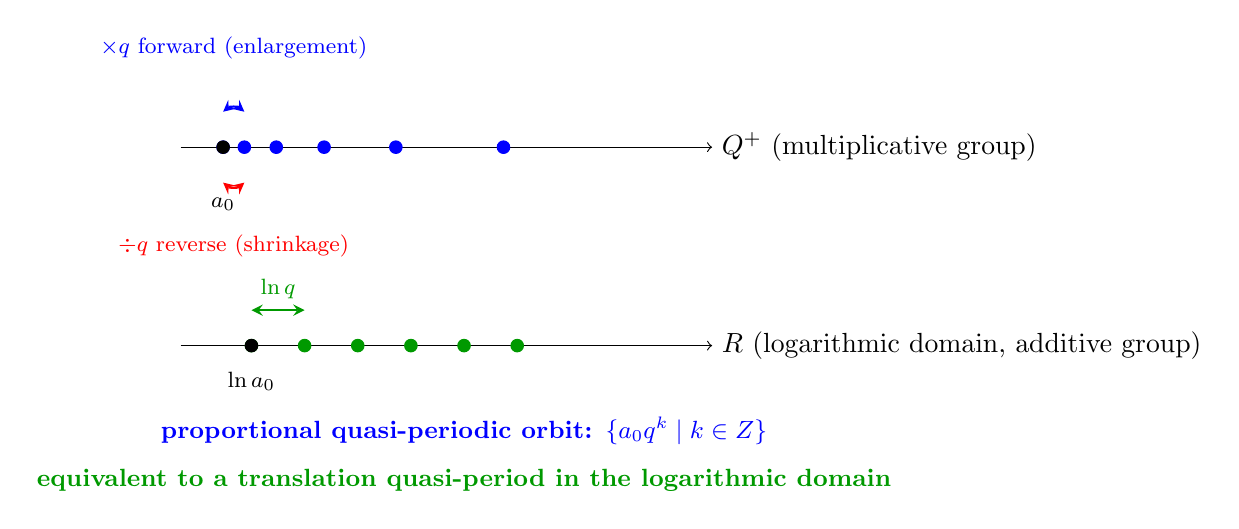
\begin{tikzpicture}[scale=0.9]
    \draw[->] (0,0) -- (7.5,0) node[right] {$\mathbb{Q}^+$ (multiplicative group)};
    \foreach \i in {0,1,...,5} {
        \filldraw[blue] ({0.6*pow(1.5,\i)}, 0) circle (2.5pt);
    }
    \draw[<->, blue, thick, >=stealth] (0.6, 0.5) to[bend left=40] (0.9, 0.5);
    \node[blue, font=\footnotesize] at (0.75, 1.4) {$\times q$ forward (enlargement)};
    \draw[<->, red, thick, >=stealth] (0.6, -0.5) to[bend right=40] (0.9, -0.5);
    \node[red, font=\footnotesize] at (0.75, -1.4) {$\div q$ reverse (shrinkage)};
    \filldraw[black] (0.6,0) circle (2.5pt);
    \node[font=\footnotesize] at (0.6, -0.8) {$a_0$};

    \draw[->] (0,-2.8) -- (7.5,-2.8) node[right] {$\mathbb{R}$ (logarithmic domain, additive group)};
    \foreach \i in {0,1,...,5} {
        \filldraw[green!60!black] ({1.0 + \i*0.75}, -2.8) circle (2.5pt);
    }
    \draw[<->, green!60!black, thick, >=stealth] (1.0, -2.3) -- (1.75, -2.3);
    \node[green!60!black, font=\footnotesize] at (1.375, -2.0) {$\ln q$};
    \filldraw[black] (1.0,-2.8) circle (2.5pt);
    \node[font=\footnotesize] at (1.0, -3.3) {$\ln a_0$};

    \node[font=\small\bfseries, blue] at (4, -4.0) {proportional quasi-periodic orbit: $\{a_0 q^k \mid k\in\mathbb{Z}\}$};
    \node[font=\small\bfseries, green!60!black] at (4, -4.7) {equivalent to a translation quasi-period in the logarithmic domain};
\end{tikzpicture}
\caption{The proportional direction structure of the rationals $\mathbb{Q}^+$ (upper figure) and its equivalent translation direction in the logarithmic domain (lower figure). With $1$ as the multiplicative centre of symmetry, multiplication by $q$ and division by $q$ form a forward--reverse directional duality.}
\label{fig:rational_direction}
\end{figure}
\section{\texorpdfstring{The reals $\mathbb{R}$: the topological basis of quasi-periodic orbits}{The reals R: the topological basis of quasi-periodic orbits}}

\subsection{\texorpdfstring{Determination requirement}{Determination requirement}}

When the rotation angle is incommensurable, $\theta/(2\pi) \notin \mathbb{Q}$, the orbit is dense on $U(1)$ but does not close. This `denseness' is a topological concept and can be formulated rigorously only in a complete space. Moreover, the continuous translation orbit $x(t) = x_0 + vt$ requires $\mathbb{R}$ as the range of the time parameter.

\subsection{\texorpdfstring{Algebraic requirement}{Algebraic requirement}}

Completeness. This is the minimal ordered-field property that makes every Cauchy sequence converge.

\subsection{\texorpdfstring{Construction of the real numbers}{Construction of the real numbers}}

\begin{definition}[Construction of the real numbers]\label{def:real_construction}
The set of real numbers $\mathbb{R}$ consists of all Dedekind cuts $L \subset \mathbb{Q}$ satisfying the following conditions:
\begin{enumerate}[label=(\arabic*)]
    \item $L \neq \emptyset$ and $L \neq \mathbb{Q}$.
    \item If $x \in L$ and $y < x$, then $y \in L$ (closed downwards).
    \item $L$ has no greatest element.
\end{enumerate}
$\mathbb{R}$ satisfies the least-upper-bound property (completeness): every non-empty subset that is bounded above has a least upper bound.
\end{definition}

\begin{theorem}[Completeness theorem for the real numbers]\label{thm:real_completeness}
$\mathbb{R}$ is the minimal ordered field in which every Cauchy sequence converges. Specifically, the following conditions are equivalent:
\begin{enumerate}[label=(\roman*)]
    \item $\mathbb{R}$ satisfies the least-upper-bound property;
    \item every Cauchy sequence in $\mathbb{R}$ converges;
    \item $\mathbb{R}$ is the completion of $\mathbb{Q}$.
\end{enumerate}
\end{theorem}

\begin{proof}
(i)$\Rightarrow$(iii): By Definition \ref{def:real_construction}, $\mathbb{R}$ consists of all Dedekind cuts of $\mathbb{Q}$, and its least-upper-bound property is guaranteed directly by the construction: the union of any non-empty family of cuts that is bounded above is again a cut, and is the least upper bound of that family. Each real number $x$ is determined by its cut $L_x$; taking an increasing sequence of rationals in $L_x$ that approaches $x$ (for example by repeated bisection), every real number is the limit of some Cauchy sequence of rationals, that is, $\mathbb{R}$ is the completion of $\mathbb{Q}$.
(i)$\Rightarrow$(ii): Let $(x_n)$ be a Cauchy sequence in $\mathbb{R}$. For each $n$, the least-upper-bound property ensures that $u_n = \sup\{x_k : k \ge n\}$ and $l_n = \inf\{x_k : k \ge n\}$ both exist; $(u_n)$ is monotonically decreasing and $(l_n)$ monotonically increasing, and by the Cauchy property $\lim_{n\to\infty}(u_n - l_n) = 0$. Monotone bounded sequences converge (again guaranteed by the least-upper-bound property); let $x = \lim u_n = \lim l_n$; then $l_n \le x_n \le u_n$ together with the squeeze property gives $x_n \to x$.
(ii)$\Rightarrow$(i): Let $A \subset \mathbb{R}$ be non-empty and bounded above by $B$. Take $a_0 \in A$ and $b_0 = B$, and construct a nested sequence of intervals $[a_n, b_n]$ recursively: put $m_n = (a_n+b_n)/2$; if $m_n$ is an upper bound for $A$, take $[a_{n+1}, b_{n+1}] = [a_n, m_n]$, otherwise take $[a_{n+1}, b_{n+1}] = [m_n, b_n]$. The endpoint sequences $(a_n),(b_n)$ are both Cauchy (the interval length is $|b_n - a_n| = 2^{-n}(b_0 - a_0) \to 0$), so by (ii) they converge to the same limit $x$. Inductively, every $b_n$ is an upper bound for $A$ while no $a_n$ is an upper bound for $A$; hence $y \le \lim b_n = x$ for every $y \in A$ (so $x$ is an upper bound), while for any upper bound $u$ there exists $y_n \in A$ with $a_n < y_n \le u$, so $x = \lim a_n \le u$ ($x$ is the least upper bound). Therefore $x = \sup A$.
\end{proof}

\subsection{\texorpdfstring{Closure of the root operation}{Closure of the root operation}}

\begin{theorem}[Real-number completeness closes the root operation]\label{thm:real_root_closure}
For every $b > 0$ and $n \in \mathbb{N}^+$, the equation $x^n = b$ has a unique positive solution $x = \sqrt[n]{b}$ in $\mathbb{R}$.
\end{theorem}

\begin{proof}
Construct the Dedekind cut $L = \{q \in \mathbb{Q} : q \le 0 \text{ or } q^n < b\}$. Verify that $L$ satisfies the three conditions for a Dedekind cut: (1) $0 \in L$ and $b+1$ is an upper bound, so $L \neq \emptyset, \mathbb{Q}$; (2) if $q \in L$ and $r < q$, then when $r\le0$ the definition of $L$ gives $r\in L$ directly, while when $r > 0$ we have $r^n < q^n < b$, so $r \in L$; (3) for any $q \in L$ with $q > 0$ one can choose $\varepsilon > 0$ sufficiently small that $(q+\varepsilon)^n < b$, so $q+\varepsilon \in L$ and $L$ has no greatest element. The real number $x$ defined by $L$ satisfies $x^n = b$. Uniqueness is guaranteed by the strict monotonicity of the power function.
\end{proof}

\subsection{\texorpdfstring{Function-theoretic features: the continuous translation equation and quasi-periods}{Function-theoretic features: the continuous translation equation and quasi-periods}}

\begin{theorem}[The group with periodic orbits of the continuous translation equation on the reals]\label{thm:translation_equation_R}
Let $f:\mathbb{R}\to Y$ be continuous and $T>0$. If
\[
f(x+T)=f(x),\qquad \forall x\in\mathbb{R},
\]
then the group with periodic orbits
\[
\operatorname{Group}_{\mathrm{period},\mathbb{R}}(f)=\{t\in\mathbb{R}: f(x+t)=f(x),\ \forall x\in\mathbb{R}\}
\]
is a closed subgroup of $\mathbb{R}$. A closed subgroup of $\mathbb{R}$ is either $\mathbb{R}$ itself or a discrete subgroup $T_0\mathbb{Z}$ ($T_0>0$).
\end{theorem}

\begin{proof}
Continuity and $f(x+T)=f(x)$ give $T\mathbb{Z}\le\operatorname{Group}_{\mathrm{period},\mathbb{R}}(f)$. The group with periodic orbits is closed under addition and under taking inverses, and by the continuity of $f$, if $t_n\in\operatorname{Group}_{\mathrm{period},\mathbb{R}}(f)$ and $t_n\to t$, then $f(x+t)=f(x)$; hence it is a closed subgroup. The classification of the closed subgroups of $\mathbb{R}$ is a standard result: if the subgroup contains arbitrarily small positive elements then it is $\mathbb{R}$, and otherwise it is the discrete subgroup $T_0\mathbb{Z}$.
\end{proof}

\begin{proposition}[Quasi-periodic orbits and completeness]\label{prop:quasi_period_R}
If $\theta/(2\pi)\notin\mathbb{Q}$, then the rotation orbit $\{e^{in\theta}\}$ is dense on $U(1)$. The rigorous formulation of denseness relies on the completeness of $\mathbb{R}$ (Theorem \ref{thm:real_completeness}): without completeness the notions of limit and closure cannot be defined.
\end{proposition}

\begin{proof}
By Kronecker's approximation theorem, $\{n\theta\bmod 2\pi\}$ is dense in $[0,2\pi)$. Denseness requires that for every $\varepsilon>0$ there is an orbit point lying in the $\varepsilon$-neighbourhood of any given point, and this relies on the existence of limits in $\mathbb{R}$, that is, on completeness.
\end{proof}

\begin{remark}[The reals make the translation equation continuous]\label{rem:real_makes_translation_continuous}
In the integers the group with periodic orbits of the translation equation is a discrete subgroup $a\mathbb{Z}$; in the reals the group with periodic orbits of the translation equation can be any closed subgroup, including the continuous group $\mathbb{R}$ itself. This is an instance of number-system extension making a function equation pass from `discrete' to `continuous'. The rotation equation $f(e^{i\theta}z)=f(z)$ still cannot be algebraised in the reals, because $e^{i\theta}$ does not belong to $\mathbb{R}$.
\end{remark}

\subsection{\texorpdfstring{Criterion theorem}{Criterion theorem}}

\begin{theorem}[Quasi-period criterion for the real numbers]\label{thm:real_quasi_period_criterion}
Let $\theta/(2\pi) \notin \mathbb{Q}$. Then the rotation orbit
\[
\mathcal{O}(z_0;\theta) = \{z_0 e^{in\theta} \mid n\in\mathbb{Z}\}
\]
is dense on $U(1)$. This denseness conclusion has a rigorous topological meaning only in $\mathbb{R}$.
\end{theorem}

\begin{proof}
By Kronecker's approximation theorem, if $\theta/(2\pi)$ is irrational then the set $\{n\theta \bmod 2\pi \mid n\in\mathbb{Z}\}$ is dense in $[0,2\pi)$. Hence the orbit points are dense on $U(1)$. The definition of denseness requires that for every $\varepsilon > 0$ there is an orbit point lying in the $\varepsilon$-neighbourhood of any given point, and this requires the completeness of the reals.
\end{proof}

\begin{corollary}[Real numbers and quasi-periods]\label{cor:real_quasi_period}
$\mathbb{R}$ is the minimal complete number system in which quasi-periodic orbits can be described but not determined in finitely many steps (deduced from Theorem \ref{thm:real_quasi_period_criterion} and Theorem \ref{thm:real_completeness}). Specifically:
\begin{enumerate}[label=(\roman*)]
    \item topological concepts such as denseness, limits and continuity hold rigorously in $\mathbb{R}$;
    \item but the rationality of a real number cannot be determined in finitely many steps---hence $\mathbb{R}$ cannot enhance the determination of finite rotation periods.
\end{enumerate}
\end{corollary}

\begin{proof}
(i) Theorem \ref{thm:real_completeness} guarantees that every Cauchy sequence in $\mathbb{R}$ converges, so topological concepts such as denseness, limits and continuity have a rigorous meaning.
(ii) Theorem \ref{thm:real_quasi_period_criterion} asserts only the denseness of the orbit corresponding to an irrational rotation angle, which is an existence description rather than a finite determination; determining the rationality of a real number requires an infinite examination of its decimal (or continued-fraction) expansion, which cannot be completed in finitely many steps, so $\mathbb{R}$ does not enhance the determination of finite rotation periods.
\end{proof}

\begin{proposition}[Effect of real-number completion on the directional structure]\label{prop:real_completion_direction}
The completeness of the reals lifts the translation direction and the proportional direction from discrete groups to continuous groups:
\begin{enumerate}[label=(\roman*)]
    \item \textbf{Continuisation of the translation direction}: the translation group is lifted from $(\mathbb{Z},+)$ to $(\mathbb{R},+)$. Translation orbits change from discrete isometric sequences of points into continuous straight lines.
    \item \textbf{Continuisation of the proportional direction}: the scaling group is lifted from the discrete subgroup $\{q^k\}$ to $(\mathbb{R}^+,\times)$. Proportional orbits are equivalent to continuous translations in the logarithmic domain.
    \item \textbf{Topological completion of the rotation direction}: the dense quasi-periodic orbits produced by incommensurable rotation angles acquire a rigorous limiting meaning in $\mathbb{R}$.
\end{enumerate}
\end{proposition}

\begin{proof}
(i) $(\mathbb{R},+)$ is the minimal continuous extension of $(\mathbb{Z},+)$ under completion: $(\mathbb{Q},+)$ embeds densely in $(\mathbb{R},+)$, and $(\mathbb{Z},+)$ is a discrete generating set for $(\mathbb{Q},+)$; hence the translation group is lifted from the integer multiples of the discrete generator $1$ to translations $x \mapsto x + t$ by a continuous parameter $t \in \mathbb{R}$, and the orbit $\{x_0 + t \mid t \in \mathbb{R}\}$ is a continuous straight line.
(ii) The exponential map $\exp: (\mathbb{R},+) \to (\mathbb{R}^+,\times)$ is a group isomorphism (see Theorem \ref{thm:log_isomorphism_conservation}), so the scaling group is lifted from the discrete subgroup $\{q^k \mid k \in \mathbb{Z}\}$ to the continuous group $(\mathbb{R}^+,\times) = \{\exp(t) \mid t \in \mathbb{R}\}$, and the proportional orbit $\{a_0 r \mid r \in \mathbb{R}^+\}$ is equivalent to a continuous translation orbit in the logarithmic domain.
(iii) By Theorem \ref{thm:real_quasi_period_criterion}, $\{n\theta \bmod 2\pi\}$ is dense in $[0,2\pi)$; topological concepts such as denseness, limits and closure depend on the completeness of $\mathbb{R}$ (Theorem \ref{thm:real_completeness}), so the dense quasi-periodic orbits of incommensurable rotations acquire a rigorous limiting meaning in $\mathbb{R}$.
\end{proof}

\begin{figure}[htbp]
\centering
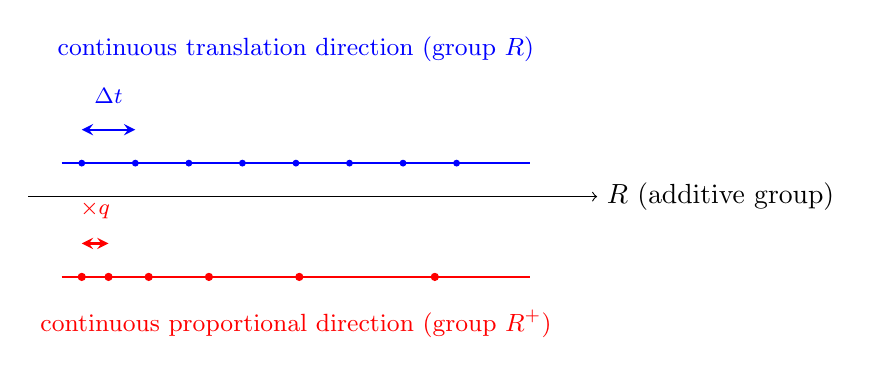
\begin{tikzpicture}[scale=0.85]
    \draw[->] (0,0) -- (8.5,0) node[right] {$\mathbb{R}$ (additive group)};
    \draw[blue, thick] (0.5,0.5) -- (7.5,0.5);
    \node[blue, font=\small] at (4, 2.2) {continuous translation direction (group $\mathbb{R}$)};
    \foreach \x in {0.8,1.6,...,7.2} {
        \filldraw[blue] (\x, 0.5) circle (1.2pt);
    }
    \draw[<->, blue, thick, >=stealth] (0.8, 1.0) -- (1.6, 1.0);
    \node[blue, font=\footnotesize] at (1.2, 1.5) {$\Delta t$};

    \draw[red, thick] (0.5,-1.2) -- (7.5,-1.2);
    \node[red, font=\small] at (4, -1.9) {continuous proportional direction (group $\mathbb{R}^+$)};
    \filldraw[red] (0.8,-1.2) circle (1.5pt);
    \filldraw[red] (1.2,-1.2) circle (1.5pt);
    \filldraw[red] (1.8,-1.2) circle (1.5pt);
    \filldraw[red] (2.7,-1.2) circle (1.5pt);
    \filldraw[red] (4.05,-1.2) circle (1.5pt);
    \filldraw[red] (6.075,-1.2) circle (1.5pt);
    \draw[<->, red, thick, >=stealth] (0.8, -0.7) -- (1.2, -0.7);
    \node[red, font=\footnotesize] at (1.0, -0.2) {$\times q$};
\end{tikzpicture}
\caption{The continuous directional structure brought about by the completion of the reals. The translation direction is lifted from the discrete group $\mathbb{Z}$ to the continuous group $\mathbb{R}$ (upper figure). The proportional direction is equivalent to continuous translation in the logarithmic domain (lower figure).}
\label{fig:real_continuous}
\end{figure}
\section{\texorpdfstring{The complex numbers $\mathbb{C}$: algebraisation of rotation periods and double periods}{The complex numbers C: algebraisation of rotation periods and double periods}}

\subsection{\texorpdfstring{Determination requirement}{Determination requirement}}

The rotation operation needs to be expressed by algebraic operations, not merely by geometric intuition. A finite rotation period $C_n$ requires the complete solution set of the algebraic equation $z^n = 1$. Moreover, double-period structures (elliptic functions) require discrete subgroups of the complex plane.

\subsection{\texorpdfstring{Algebraic requirement}{Algebraic requirement}}

The imaginary unit $i$, and algebraic closure. This is the minimal field extension that makes all polynomial equations solvable.

\subsection{\texorpdfstring{Construction of the complex numbers}{Construction of the complex numbers}}

\begin{definition}[Construction of the complex numbers]\label{def:complex_construction}
$\mathbb{C} := \mathbb{R}^2$ as a real vector space. Addition is defined componentwise:
\[
(a,b) + (c,d) := (a+c, b+d).
\]
Multiplication is defined by
\[
(a,b) \times (c,d) := (ac - bd, ad + bc).
\]
Write $i := (0,1)$; then $i^2 = (0,1) \times (0,1) = (-1,0) = -1$. Every complex number can be written as $z = a + bi$ ($a,b \in \mathbb{R}$).
\end{definition}

\begin{proposition}[The complex numbers form a field]\label{prop:complex_algebraically_closed}
$(\mathbb{C},+,\times)$ forms a field. That is:
\begin{enumerate}[label=(\roman*)]
    \item $(\mathbb{C},+)$ is an abelian group with zero element $(0,0)$;
    \item $(\mathbb{C}^{\times}, \times)$ is an abelian group with multiplicative inverse $z^{-1} = \bar{z}/|z|^2$ ($z \neq 0$);
    \item multiplication satisfies the distributive law over addition.
\end{enumerate}
\end{proposition}

\begin{proof}
(i) Addition is defined componentwise, each component being added in $\mathbb{R}$; hence associativity, commutativity, the zero element $(0,0)$ and the negative $-(a,b) = (-a,-b)$ are all inherited componentwise from the additive group structure of $\mathbb{R}$.
(ii) The commutativity and associativity of multiplication are verified by direct expansion from the definition: $(a,b)(c,d) = (ac-bd, ad+bc) = (ca-db, cb+da) = (c,d)(a,b)$; expanding associativity componentwise reduces it to the laws of operation in $\mathbb{R}$. The multiplicative identity is $(1,0)$. For $z = (a,b) \neq 0$ we have $|z|^2 = a^2+b^2 > 0$, and
\[
(a,b)\left(\frac{a}{a^2+b^2}, \frac{-b}{a^2+b^2}\right) = \left(\frac{a^2+b^2}{a^2+b^2}, \frac{-ab+ba}{a^2+b^2}\right) = (1,0),
\]
so $z^{-1} = \bar{z}/|z|^2$ is the multiplicative inverse.
(iii) The distributive law is verified by expanding componentwise from the definition:
\[
(a,b)\bigl[(c,d)+(e,f)\bigr] = (a,b)(c+e, d+f) = \bigl(a(c+e)-b(d+f), a(d+f)+b(c+e)\bigr)
\]
\[
= (ac-bd, ad+bc) + (ae-bf, af+be) = (a,b)(c,d) + (a,b)(e,f).
\]
\end{proof}

\begin{proposition}[Completeness of the complex numbers]\label{prop:complex_completeness}
As a metric space, $\mathbb{C} \cong \mathbb{R}^2$ is complete: a Cauchy sequence $\{z_n = a_n + ib_n\}$ in $\mathbb{C}$ converges if and only if both the real-part sequence $\{a_n\}$ and the imaginary-part sequence $\{b_n\}$ converge in $\mathbb{R}$.
\end{proposition}

\begin{proof}
By the completeness of $\mathbb{R}$ (Theorem \ref{thm:real_completeness}), $\{a_n\}$ and $\{b_n\}$ converge to $a, b \in \mathbb{R}$ respectively. Then $z_n \to a + bi \in \mathbb{C}$. Conversely, if $z_n \to z = a+bi$, then $|a_n - a| \le |z_n - z| \to 0$ and $|b_n - b| \le |z_n - z| \to 0$.
\end{proof}

\begin{remark}[The fundamental theorem of algebra (algebraic closure)]\label{rem:fta}
The complex field $\mathbb{C}$ is \textbf{algebraically closed}: every non-zero polynomial with complex coefficients has at least one root in $\mathbb{C}$. This is the fundamental theorem of algebra; its standard proof requires complex analysis (Liouville's theorem or the argument principle) or topological/algebraic methods, which lie beyond the deductive scope of `number-system extension' in this chapter, so it is cited here as a standard result without proof. In what follows this chapter uses only its weaker corollary---`a polynomial of degree $n$ has at most $n$ roots'---and that conclusion can be proved directly on any field by the factor theorem (see the proof of Theorem \ref{thm:complex_finite_rotation_criterion}); it does not depend on the full strength of the fundamental theorem of algebra.
\end{remark}

\subsection{\texorpdfstring{Algebraisation of rotation}{Algebraisation of rotation}}

\begin{theorem}[Algebraisation of complex rotation]\label{thm:complex_rotation_algebraization}
The unit circle
\[
S^1 = \{z \in \mathbb{C} \mid |z| = 1\}
\]
forms a group under complex multiplication, isomorphic to $U(1)$. The algebraic realisation of the rotation $R_\theta$ is
\[
R_\theta(z) = e^{i\theta} z,
\]
where $e^{i\theta} = \cos\theta + i\sin\theta$ (Euler's formula).
\end{theorem}

\begin{proof}
$|e^{i\theta} z| = |e^{i\theta}| \cdot |z| = 1 \cdot |z| = |z|$, so rotation preserves the modulus. Since $e^{i(\theta_1 + \theta_2)} = e^{i\theta_1} e^{i\theta_2}$, the rotation group is isomorphic to $U(1)$. Euler's formula follows by comparing the power-series expansion of $e^{i\theta}$ with the power-series expansion of $\cos\theta, \sin\theta$.
\end{proof}

\subsection{\texorpdfstring{Function-theoretic features: the rotation equation and roots of unity}{Function-theoretic features: the rotation equation and roots of unity}}

\begin{theorem}[The group with periodic orbits of the rotation equation on the complex numbers]\label{thm:rotation_equation_C}
Let $f:\mathbb{C}^\times\to Y$ and $\theta\in\mathbb{R}$. If
\[
f(e^{i\theta}z)=f(z),\qquad \forall z\in\mathbb{C}^\times,
\]
then the group with periodic orbits
\[
\operatorname{Group}_{\mathrm{period},U(1)}(f)=\{e^{i\theta}\in U(1): f(e^{i\theta}z)=f(z),\ \forall z\in\mathbb{C}^\times\}
\]
is a subgroup of $U(1)$. If $\theta/(2\pi)=p/q$ in lowest terms, then $e^{i\theta}$ has order $q$, and $\langle e^{i\theta}\rangle\cong C_q\le\operatorname{Group}_{\mathrm{period},U(1)}(f)$.
\end{theorem}

\begin{proof}
Iterating $f(e^{i\theta}z)=f(z)$ in both directions gives $f(e^{in\theta}z)=f(z)$ for every $n\in\mathbb{Z}$, so $\langle e^{i\theta}\rangle\le\operatorname{Group}_{\mathrm{period},U(1)}(f)$. If $\theta/(2\pi)=p/q$ in lowest terms, then $e^{i\theta}$ is a $q$-th root of unity of order $q$, generating $C_q$.
\end{proof}

\begin{corollary}[The unit-root equation and finite rotation periods]\label{cor:unit_root_C}
The equation $z^n=1$ has exactly $n$ solutions in $\mathbb{C}$, forming the cyclic group $C_n$. This is the algebraic prototype of the rotation equation $f(e^{i\theta}z)=f(z)$ at $\theta=2\pi/n$: taking $f(z)=z^n$, we have $f(e^{2\pi i/n}z)=z^n=f(z)$.
\end{corollary}

\begin{figure}[htbp]
    \centering
    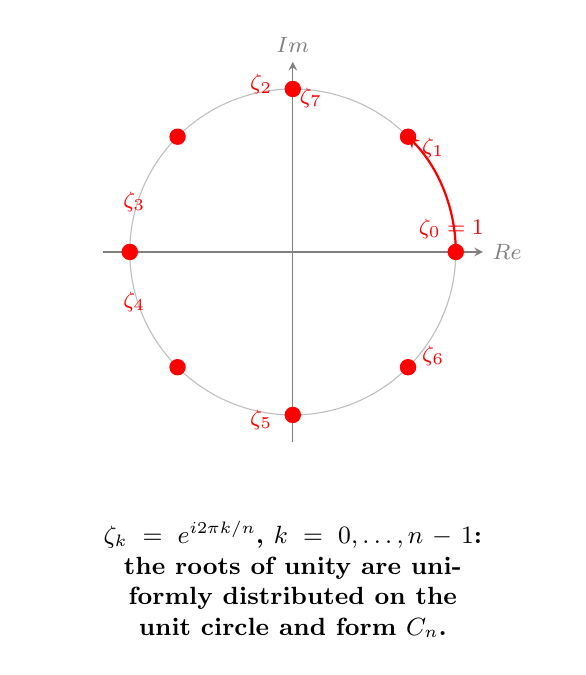
\begin{tikzpicture}[scale=1.15,>=stealth]
        \draw[gray!50, thin] (0,0) circle (1.8);
        \draw[->, gray] (-2.1,0) -- (2.1,0) node[right, font=\footnotesize] {$\operatorname{Re}$};
        \draw[->, gray] (0,-2.1) -- (0,2.1) node[above, font=\footnotesize] {$\operatorname{Im}$};

        \foreach \k in {0,1,...,7} {
            \filldraw[red] ({360/8*\k}:1.8) circle (2.4pt);
        }
        \draw[->, red, thick] (1.8,0) arc (0:45:1.8);
        \node[red, font=\footnotesize] at (1.55,1.15) {$\zeta_1$};
        \node[red, font=\footnotesize] at (-0.35,1.85) {$\zeta_2$};
        \node[red, font=\footnotesize] at (-1.75,0.55) {$\zeta_3$};
        \node[red, font=\footnotesize] at (-1.75,-0.55) {$\zeta_4$};
        \node[red, font=\footnotesize] at (-0.35,-1.85) {$\zeta_5$};
        \node[red, font=\footnotesize] at (1.55,-1.15) {$\zeta_6$};
        \node[red, font=\footnotesize] at (1.75,0.25) {$\zeta_0=1$};
        \node[red, font=\footnotesize] at (0.2,1.7) {$\zeta_7$};

        \node[font=\small\bfseries, text width=6.5cm, align=center, below=0.3cm] at (0,-2.6)
            {$\zeta_k=e^{i2\pi k/n}$, $k=0,\dots,n-1$:\\ the roots of unity are uniformly distributed on the unit circle and form $C_n$.};
    \end{tikzpicture}
    \caption{The geometric distribution of the $n$-th roots of unity in the complex numbers (taking $n=8$ as an example). The $n$ solutions $\zeta_k=e^{2\pi ik/n}$ are equally spaced on the unit circle and form the cyclic group $C_n$ of order $n$. This is the algebraic prototype of finite rotation periods in the complex field (Theorem \ref{thm:complex_finite_rotation_criterion}); the special case $n=4$ in the figure is the fourth-order rotation orbit of Figure \ref{fig:complex_rotation_i}.}
    \label{fig:unit_roots_Cn}
\end{figure}

\begin{proof}
By Theorem \ref{thm:complex_finite_rotation_criterion}, the solution set of $z^n=1$ is $\{e^{2\pi ik/n}:k=0,\dots,n-1\}$, forming $C_n$. Taking $f(z)=z^n$, we have $f(e^{2\pi i/n}z)=(e^{2\pi i/n}z)^n=z^n=f(z)$.
\end{proof}

\begin{remark}[The complex numbers make the rotation equation algebraic]\label{rem:complex_makes_rotation_algebraic}
In the reals the rotation equation $f(e^{i\theta}z)=f(z)$ has no algebraic carrier, because $e^{i\theta}$ does not belong to $\mathbb{R}$. In the complex numbers the imaginary unit $i$ makes $e^{i\theta}$ an algebraic object, the rotation equation can be algebraised, and the group with periodic orbits $C_n$ of a finite rotation period is characterised exactly by the unit-root equation $z^n=1$. This is the key step by which number-system extension makes a function equation pass from `non-algebraisable' to `algebraisable'.
\end{remark}
\subsection{\texorpdfstring{Criterion theorem}{Criterion theorem}}

\begin{theorem}[Algebraic criterion for finite rotational periods]\label{thm:complex_finite_rotation_criterion}
The equation
\[
z^n = 1
\]
has exactly $n$ solutions in $\mathbb{C}$:
\[
\zeta_k = e^{2\pi i k/n},\qquad k = 0, 1, \dots, n-1.
\]
These $n$ solutions form the cyclic group $C_n$ of order $n$. They are the algebraic prototype of finite rotation periods.
\end{theorem}

\begin{proof}
First we prove that the solution set has exactly $n$ elements. Since $\mathbb{C}$ is a field, $z^n - 1$ is a non-zero polynomial of degree $n$, and by the factor theorem (each root $\alpha$ corresponds to a factor $(z-\alpha)$, and each extraction of a factor lowers the degree by $1$) it has at most $n$ roots. On the other hand, for $k = 0, 1, \dots, n-1$, put $\zeta_k = e^{2\pi i k/n}$; then
\[
\zeta_k^n = e^{2\pi i k} = \cos(2\pi k) + i\sin(2\pi k) = 1,
\]
and when $k \neq l$ we have $\zeta_k/\zeta_l = e^{2\pi i(k-l)/n} \neq 1$ (since $0 < |k-l| < n$), so $\zeta_0, \dots, \zeta_{n-1}$ are pairwise distinct, giving $n$ roots. Hence the solution set is exactly $\{\zeta_0, \dots, \zeta_{n-1}\}$.
Next we prove that these $n$ solutions form a cyclic group: closure under multiplication $\zeta_k \cdot \zeta_l = e^{2\pi i(k+l)/n} = \zeta_{k+l \bmod n}$; the identity element $\zeta_0 = 1$; inverses $\zeta_k^{-1} = e^{-2\pi i k/n} = \zeta_{n-k}$ (for $k = 0$, $\zeta_0^{-1} = \zeta_0$). Since $\zeta_1 = e^{2\pi i/n}$ generates the whole set ($\zeta_k = \zeta_1^k$), these $n$ solutions form the cyclic group $C_n$ of order $n$.
\end{proof}

\begin{theorem}[Period-lattice criterion for double-period structure]\label{thm:complex_double_period}
The discrete subgroup of $\mathbb{C}$
\[
\Lambda = \omega_1 \mathbb{Z} + \omega_2 \mathbb{Z},\qquad \omega_1/\omega_2 \notin \mathbb{R},
\]
is the period lattice of double-periodic functions (elliptic functions). Every elliptic function with period lattice $\Lambda$ satisfies
\[
f(z + \omega_1) = f(z), \qquad f(z + \omega_2) = f(z).
\]
The two independent periods $\omega_1, \omega_2$ correspond to two translation directions respectively.
\end{theorem}

\begin{proof}
$\Lambda$ is a discrete additive subgroup of $\mathbb{C}$ of rank $2$ (because $\omega_1/\omega_2 \notin \mathbb{R}$ guarantees that the two directions are linearly independent). The quotient space $\mathbb{C}/\Lambda$ is a compact complex manifold (an elliptic curve). The Weierstrass $\wp$ function is the typical elliptic function on the period lattice $\Lambda$.
\end{proof}

\subsection{\texorpdfstring{The involution of the centre of symmetry $i$}{The involution of the centre of symmetry i}}

\begin{definition}[The involution of the centre of symmetry $i$]\label{def:complex_i_involution}
On $\mathbb{C}^{\times}$ define the map
\[
\sigma_i: \mathbb{C}^{\times} \to \mathbb{C}^{\times}, \quad \sigma_i(z) = i \cdot z^{-1}.
\]
Writing $z$ in polar form $z = re^{i\varphi}$, from $z^{-1} = r^{-1}e^{-i\varphi}$ this operation becomes
\[
\sigma_i(re^{i\varphi}) = i \cdot r^{-1} e^{-i\varphi} = r^{-1} e^{i(\pi/2 - \varphi)}.
\]
This operation comprises simultaneously \textbf{scaling} (taking the reciprocal of the modulus, $r \mapsto r^{-1}$) and a reflection of the argument about the $\pi/4$ direction ($\varphi \mapsto \pi/2 - \varphi$).
\end{definition}

\begin{proposition}[Basic properties of the involution $\sigma_i$]\label{prop:complex_i_involution_properties}
\begin{enumerate}[label=(\roman*)]
    \item $\sigma_i$ is an involution: $\sigma_i \circ \sigma_i = \text{id}_{\mathbb{C}^{\times}}$.
    \item The fixed points of $\sigma_i$ satisfy $z^2 = i$, that is, $z = \pm \frac{\sqrt{2}}{2}(1+i)$.
    \item $\sigma_i = R_{\pi/2} \circ \sigma_1$, where $R_{\pi/2}(z) = iz$ is rotation through $90^\circ$ and $\sigma_1(z) = z^{-1}$ is the taking-the-inverse involution.
\end{enumerate}
\end{proposition}

\begin{proof}
(i) $\sigma_i(\sigma_i(z)) = i \cdot (i \cdot z^{-1})^{-1} = i \cdot (-i \cdot z) = z$ (note that $(i \cdot w)^{-1} = -i \cdot w^{-1}$ because $i \cdot (-i) = 1$).
(ii) $\sigma_i(z) = z \iff i \cdot z^{-1} = z \iff z^2 = i \iff z = \pm e^{i\pi/4}$.
(iii) $R_{\pi/2}(\sigma_1(z)) = i \cdot z^{-1} = \sigma_i(z)$.
\end{proof}

\begin{example}[Unification of scaling and rotation in the complex power map]\label{ex:complex_power_scaling_rotation}
Consider the complex power function $f_n: \mathbb{C}^{\times} \to \mathbb{C}^{\times}, z \mapsto z^n$ ($n \in \mathbb{N}^+$). Put $z = re^{i\theta}$; then
\[
f_n(z) = r^n e^{in\theta}.
\]
This map acts simultaneously on the scaling dimension (modulus $r \mapsto r^n$) and on the rotation dimension (argument $\theta \mapsto n\theta$). If $|z|=1$, then $f_n$ is an $n$-fold endomorphism of the rotation group $U(1)$. The complex power operation unifies the proportional direction and the rotation direction in a single operation.

Explicit computation: take $z = 2 e^{i\pi/4}$ and $n = 3$; then
\[
f_3(z) = 2^3\, e^{3 \cdot i\pi/4} = 8\, e^{3\pi i/4} = 8\left(-\frac{\sqrt{2}}{2} + i\frac{\sqrt{2}}{2}\right) = -4\sqrt{2} + 4\sqrt{2}\,i.
\]
The modulus $|z| = 2$ is enlarged to $|f_3(z)| = 8$ (proportional direction, scaling $r \mapsto r^3$), and the argument $\pi/4$ is rotated to $3\pi/4$ (rotation direction, $\theta \mapsto 3\theta$); the two are accomplished simultaneously in one operation, verifying that the complex power realises scaling and rotation at once.
\end{example}

\begin{figure}[htbp]
\centering
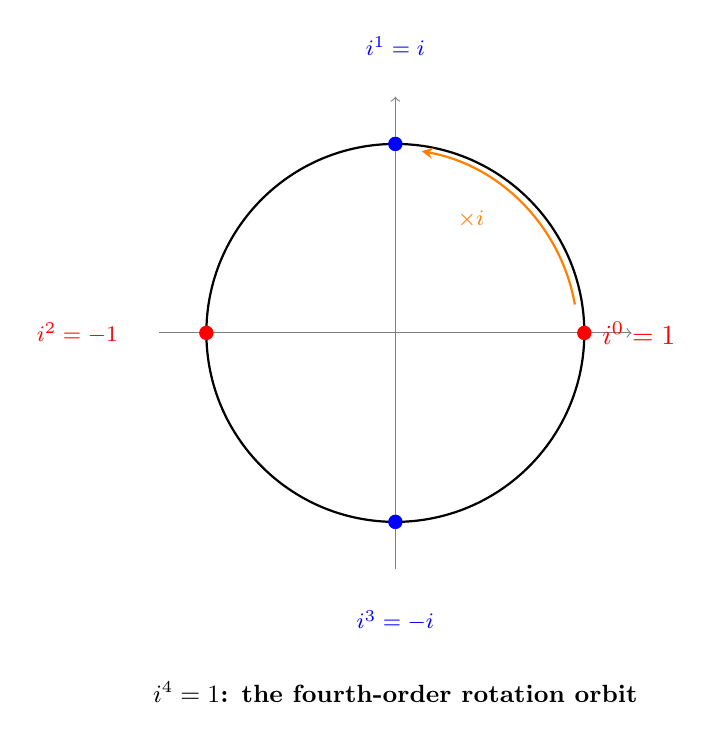
\begin{tikzpicture}[scale=1.2]
    \draw[thick] (0,0) circle (2.0);
    \draw[->, gray] (-2.5,0) -- (2.5,0);
    \draw[->, gray] (0,-2.5) -- (0,2.5);
    \filldraw[red] (2,0) circle (2pt) node[right=3pt] {$i^0=1$};
    \filldraw[blue] (0,2) circle (2pt) node[above=1cm, font=\footnotesize] {$i^1=i$};
    \filldraw[red] (-2,0) circle (2pt) node[left=1cm, font=\footnotesize] {$i^2=-1$};
    \filldraw[blue] (0,-2) circle (2pt) node[below=1cm, font=\footnotesize] {$i^3=-i$};
    \draw[->, thick, >=stealth, orange] (1.9, 0.3) arc (10:80:2.0);
    \node[orange, font=\footnotesize] at (0.8, 1.2) {$\times i$};
    \node[font=\small\bfseries] at (0, -3.8) {$i^4=1$: the fourth-order rotation orbit};
\end{tikzpicture}
\caption{The rotation direction generated by complex multiplication $z \mapsto iz$: multiplication by $i$ is rotation through $90^\circ$, and the fourth power returns to the starting point, forming a fourth-order rotation orbit.}
\label{fig:complex_rotation_i}
\end{figure}

\begin{definition}[The fourfold discrete skeleton of the unit circle]\label{def:unit_circle_fourfold_skeleton}
The fourfold discrete skeleton of the unit circle $S^1=\{z\in\mathbb{C}\mid |z|=1\}$ is defined as
\[
C_4=\mu_4=\{1,i,-1,-i\}=\{i^k\mid k=0,1,2,3\},
\]
in which the phase and the algebraic role of each element are
\[
1=e^{i0}\ (\text{multiplicative identity, the fixed point of rotation}),\qquad
i=e^{i\pi/2}\ (\text{quarter turn}),
\]
\[
-1=e^{i\pi}=i^2\ (\text{half turn, that is, sign flip}),\qquad
-i=e^{i3\pi/2}=i^3\ (\text{three-quarter turn}).
\]
This set forms the cyclic group $C_4$ of order $4$ under complex multiplication: it is the finite rotation orbit generated by $i$ (Figure \ref{fig:complex_rotation_i}), and it is also the complete solution set of the unit-root equation $z^4=1$ in $\mathbb{C}$ (Theorem \ref{thm:complex_finite_rotation_criterion} with $n=4$; see also Corollary \ref{cor:unit_root_C}). Its continuous refinement gives the whole unit circle:
\[
S^1=\{e^{i\theta}\mid\theta\in\mathbb{R}\}\cong U(1).
\]
$C_4$ is the smallest discrete skeleton of $S^1$ that contains $i$: the set $\{1,-1\}$ is its subgroup of order $2$, and the adjunction of $i$ raises the skeleton from order $2$ to order $4$.
\end{definition}

\begin{proposition}[The sign system is the projection of the rotation group at $180^\circ$, and $i$ refines it to $C_4$]\label{prop:sign_as_half_turn_projection}
Under the embedding of the reals $\mathbb{R}\hookrightarrow\mathbb{C}$, $x\mapsto x+0i$:
\begin{enumerate}[label=(\roman*)]
    \item The sign system $\{\pm1\}$ forms the cyclic group $C_2$ of order $2$ under multiplication, and is a subgroup of the multiplicative group of $\mathbb{R}$ (item (ii) of Proposition \ref{prop:complex_algebraically_closed}).
    \item The map $\pi_1:\mu_4\to\{\pm1\}$, $\pi_1(e^{i\theta})=e^{i2\theta}$, is a surjective group homomorphism; it pairs up the four phases $0,\pi/2,\pi,3\pi/2$ and presses them onto the two phases $0,\pi$, so that $\pi_1(\mu_4)=\{\pm1\}$ is precisely the projection of the rotation group at $180^\circ$ (the half turn). Its kernel is $\ker\pi_1=\{\pm1\}$, and the first isomorphism theorem gives $\mu_4/\{\pm1\}\cong\{\pm1\}$.
    \item The real sign system $\{\pm1\}$ is the image of the rotation group under the projection at $180^\circ$: $\mu_4/\{\pm1\}\cong\{\pm1\}$ shows that it is exactly the quotient of the fourfold rotation skeleton by the half-turn projection; equivalently, $\mathbb{R}\cap\mu_4=\{\pm1\}$, that is, only two real elements of the fourfold skeleton are visible on the real axis.
    \item Adjoining $i$ refines $\{\pm1\}\cong C_2$ to $\mu_4\cong C_4$, and $C_2=\langle-1\rangle$ is the unique subgroup of order $2$ of $C_4$; continuous refinement (completing the discrete phases to arbitrary real phases) then gives $S^1\cong U(1)$.
\end{enumerate}
\end{proposition}

\begin{proof}
(i) $\{\pm1\}$ is closed under multiplication ($1\cdot1=1$, $(-1)\cdot(-1)=1$, $1\cdot(-1)=-1$), contains the identity $1$, and satisfies $(-1)^{-1}=-1$, so it is a group; $\langle-1\rangle$ has order $2$, hence is isomorphic to $C_2$, and it is a subgroup of $\mathbb{R}^\times$.

(ii) Define $\pi_1(e^{i\theta})=e^{i2\theta}$. For $e^{i\theta_1},e^{i\theta_2}\in\mu_4$ we have $\pi_1(e^{i\theta_1}e^{i\theta_2})=\pi_1(e^{i(\theta_1+\theta_2)})=e^{i2(\theta_1+\theta_2)}=\pi_1(e^{i\theta_1})\pi_1(e^{i\theta_2})$, so $\pi_1$ is a group homomorphism; the images of the four phases are $e^{i0}=1$, $e^{i\pi}=-1$, $e^{i2\pi}=1$, $e^{i3\pi}=-1$, so the image is $\{\pm1\}$; the kernel consists of the elements whose doubled phase is $0$, namely $e^{i0}=1$ and $e^{i\pi}=-1$, so $\ker\pi_1=\{\pm1\}$, and the first isomorphism theorem gives $\mu_4/\{\pm1\}\cong\{\pm1\}$.

(iii) By (ii), the kernel of the half-turn projection is $\{\pm1\}$ and its image is $\{\pm1\}$; moreover the elements of $\mu_4$ that lie in $\mathbb{R}$ are exactly $\pm1$ (since $i,-i$ have imaginary part $\pm1\neq0$), so $\mathbb{R}\cap\mu_4=\{\pm1\}$.

(iv) Since $i^2=-1$ and $i^4=1$, the element $i$ has order $4$ in $\mathbb{C}^{\times}$ and generates $\mu_4=\langle i\rangle\cong C_4$, in which $\{\pm1\}=\langle-1\rangle$ is a subgroup of order $2$; the order of a subgroup of $C_4$ divides $4$, so the subgroup of order $2$ is unique. Completing the discrete phases $k\pi/2$ to arbitrary real phases $\theta$ gives $S^1=\{e^{i\theta}\mid\theta\in\mathbb{R}\}$; for the isomorphism with $U(1)$ see Theorem \ref{thm:complex_rotation_algebraization}.
\end{proof}

\begin{remark}[The conditions under which `the sign is a rotation by $\pi$' holds]\label{rem:sign_versus_additive_reflection}
The assertion in the preceding proposition that `a sign flip is a half turn' holds only after the embedding $\mathbb{R}\subset\mathbb{C}$; two structures must here be kept clearly apart, lest the text appear to conflict with the three centres of symmetry $0,1,i$ established in this chapter:
\begin{itemize}
    \item Considered on $\mathbb{R}$ alone, $x\mapsto-x$ is the \textbf{additive reflection with centre $0$}: it is the involutive automorphism $\sigma_0$ of the additive group, its fixed point is $0$, and it generates $C_2$ (item (ii) of Proposition \ref{prop:integer_symmetry_direction_period}); it is \textbf{not} a rotation in the complex plane, because $\mathbb{R}$ contains no carrier of the phase $e^{i\pi}$ (see Remark \ref{rem:complex_makes_rotation_algebraic}).
    \item In $\mathbb{C}$, and only there, $-1=e^{i\pi}$ is the half turn on the unit circle, that is, the flip in multiplication with centre $1$ and phase $\pi$. The relation between the two is given by the restriction map: the restriction of the additive reflection $\sigma_0$ to $\{\pm1\}\subset\mathbb{C}$ is exactly multiplication by $-1$, that is, the action of $e^{i\pi}$ on the real axis; in other words, the additive reflection is the restriction of the half turn to the real axis, whilst the half turn is the phase realisation of the additive reflection in $\mathbb{C}$.
    \item Accordingly, the division of labour amongst the three centres of symmetry is: the additive centre $0$ ($\sigma_0$, symmetry type additive reflection), the multiplicative centre $1$ ($\sigma_1$, symmetry type taking the multiplicative inverse, Definition \ref{def:rational_involution}), and the phase centre $i$ ($\sigma_i$, Definition \ref{def:complex_i_involution}). The sign system $\{\pm1\}$ is not an additional centre of symmetry: it is the common image of $\sigma_0$ and of the half turn on the real axis.
\end{itemize}
\end{remark}

\section{\texorpdfstring{The quaternions $\mathbb{H}$: algebraisation of three-dimensional rotation periods}{The quaternions H: algebraisation of three-dimensional rotation periods}}

\subsection{\texorpdfstring{Determination requirement}{Determination requirement}}

A two-dimensional rotation needs only one angle parameter, corresponding to $U(1)$, which is an abelian group. A three-dimensional rotation needs three parameters, corresponding to $SO(3)$, which is a non-abelian group. Complex numbers can express only planar rotations and cannot express the non-commutativity of three-dimensional rotations.

\subsection{\texorpdfstring{Algebraic requirement}{Algebraic requirement}}

A non-commutative multiplication structure. This is the minimal algebraic extension that makes three-dimensional rotations algebraisable.

\subsection{\texorpdfstring{Construction of the quaternions}{Construction of the quaternions}}

\begin{definition}[Construction of the quaternions]\label{def:quaternion_construction}
$\mathbb{H} := \mathbb{R}^4$ as a real vector space, with basis elements denoted $\{1,i,j,k\}$. Multiplication is extended bilinearly from the following relations:
\[
i^2 = j^2 = k^2 = ijk = -1,
\]
together with the relations derived from them: $ij = k, ji = -k$, $jk = i, kj = -i$, $ki = j, ik = -j$.
For $q = a + bi + cj + dk$, define the conjugate $\bar{q} = a - bi - cj - dk$, the norm $|q| = \sqrt{q\bar{q}} = \sqrt{a^2+b^2+c^2+d^2}$, and the inverse $q^{-1} = \bar{q}/|q|^2$ ($q \neq 0$).
\end{definition}

\begin{proposition}[Algebraic properties of quaternions]\label{prop:quaternion_properties}
\begin{enumerate}[label=(\roman*)]
    \item $\mathbb{H}$ is a division algebra (a division ring): every non-zero element has a multiplicative inverse, but multiplication is not commutative.
    \item The group of unit quaternions $S^3 = \{q \in \mathbb{H} : |q| = 1\}$ forms a non-commutative Lie group under quaternion multiplication, isomorphic to $SU(2)$.
    \item Through the conjugation action $\rho_q(v) = q v q^{-1}$ (with $v$ a purely imaginary quaternion), $S^3$ realises rotations in three-dimensional space. The map $q \mapsto \rho_q$ gives the double covering $SU(2) \to SO(3)$.
\end{enumerate}
\end{proposition}

\begin{proof}
(i) For $q = a + bi + cj + dk \neq 0$, from $q\bar{q} = a^2+b^2+c^2+d^2 = |q|^2 > 0$ we get that $q^{-1} = \bar{q}/|q|^2$ satisfies $q q^{-1} = 1$, so every non-zero element has a multiplicative inverse; and since $ij = k \neq -k = ji$, multiplication is not commutative, so $\mathbb{H}$ is a division algebra (a division ring).
(ii) First we prove the multiplicativity of the norm $|q_1 q_2| = |q_1|\,|q_2|$: $|q_1 q_2|^2 = q_1 q_2 \overline{q_1 q_2} = q_1 q_2 \bar{q}_2 \bar{q}_1 = q_1 |q_2|^2 \bar{q}_1 = |q_1|^2 |q_2|^2$. Hence $|q_1|=|q_2|=1 \Rightarrow |q_1 q_2|=1$ and $|q^{-1}| = |\bar{q}|/|q|^2 = 1$, so $S^3$ is closed under multiplication and contains the identity element and inverses, and is a group; it is a smooth closed submanifold of $\mathbb{H}^\times$ whose multiplication is not commutative, so it is a non-commutative Lie group. The isomorphism $S^3 \cong SU(2)$ is given by $a+bi+cj+dk \mapsto \begin{pmatrix} a+bi & c+di \\ -c+di & a-bi \end{pmatrix}$, since this matrix satisfies $|q|^2 = \det M$ and $M M^\dagger = (a^2+b^2+c^2+d^2)I$, so $|q|=1$ if and only if $M \in SU(2)$.
(iii) By Theorem \ref{thm:quaternion_rotation_criterion}, the conjugation action $\rho_q(v) = q v q^{-1}$ preserves the modulus and preserves the purely imaginary space, so it is a rotation of $\mathbb{R}^3$, and $\rho_q = \rho_{-q}$ gives the double covering $SU(2) \to SO(3)$.
\end{proof}

\begin{remark}[Comparison of quaternions with complex numbers]\label{rem:quaternion_vs_complex}
The quaternions $\mathbb{H}$ are the non-commutative extension of the complex numbers $\mathbb{C}$:
\begin{itemize}
    \item $\mathbb{C}$ has only one imaginary unit ($i$), whereas $\mathbb{H}$ has three ($i,j,k$);
    \item the rotation group $U(1)$ of $\mathbb{C}$ is abelian, whereas the rotation group $SU(2)$ of $\mathbb{H}$ is non-abelian;
    \item the roots of unity $\zeta_n$ of $\mathbb{C}$ form the cyclic group $C_n$, whereas the classification of the finite subgroups of $\mathbb{H}$ is richer (cyclic, dihedral, tetrahedral, octahedral and icosahedral groups).
\end{itemize}
\end{remark}

\begin{figure}[htbp]
    \centering
    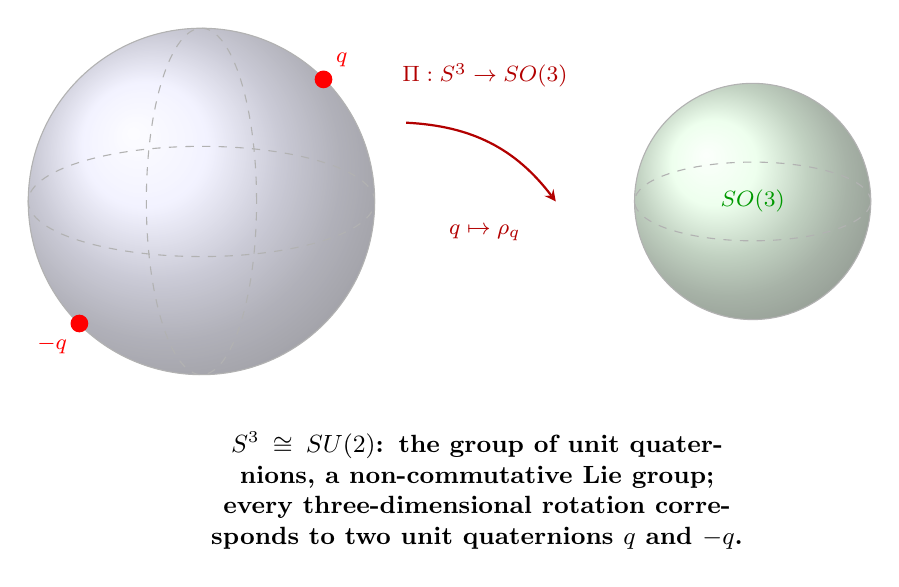
\begin{tikzpicture}[scale=1.0,>=stealth]
        \shade[ball color=blue!12, opacity=0.55] (0,0) circle (2.2);
        \draw[gray!60, thin] (0,0) circle (2.2);
        \draw[gray!60, dashed, thin] (0,0) ellipse (2.2 and 0.7);
        \draw[gray!60, dashed, thin] (0,0) ellipse (0.7 and 2.2);

        \filldraw[red] (1.55,1.55) circle (3pt);
        \node[red, font=\footnotesize, above right=1pt] at (1.55,1.55) {$q$};
        \filldraw[red] (-1.55,-1.55) circle (3pt);
        \node[red, font=\footnotesize, below left=1pt] at (-1.55,-1.55) {$-q$};

        \draw[->, thick, red!70!black] (2.6,1.0) to[bend left=25] (4.5,0);
        \node[red!70!black, font=\footnotesize, align=center] at (3.6, 1.6)
            {$\Pi:S^3\to SO(3)$};
        \node[red!70!black, font=\footnotesize, align=center] at (3.6, -0.4)
            {$q\mapsto\rho_q$};

        \shade[ball color=green!15, opacity=0.6] (7.0,0) circle (1.5);
        \draw[gray!60, thin] (7.0,0) circle (1.5);
        \draw[gray!60, dashed, thin] (7.0,0) ellipse (1.5 and 0.5);
        \node[green!60!black, font=\footnotesize] at (7.0,0) {$SO(3)$};

        \node[font=\small\bfseries, text width=7.5cm, align=center, below=2.8cm] at (3.5,0)
            {$S^3\cong SU(2)$: the group of unit quaternions, a non-commutative Lie group;\\ every three-dimensional rotation corresponds to two unit quaternions $q$ and $-q$.};
    \end{tikzpicture}
    \caption{The quaternion unit sphere $S^3\cong SU(2)$ and its double covering of $SO(3)$. $q$ and $-q$ correspond to the same three-dimensional rotation, and the kernel of $\Pi:S^3\to SO(3)$ is $\{\pm 1\}$. This is the algebraised realisation of three-dimensional rotation periods in the quaternion field (Theorem \ref{thm:quaternion_rotation_criterion}).}
    \label{fig:quaternion_S3_cover}
\end{figure}
\subsection{\texorpdfstring{Criterion theorem}{Criterion theorem}}

\begin{theorem}[Algebraisation criterion for three-dimensional rotation]\label{thm:quaternion_rotation_criterion}
The group of unit quaternions $S^3$ realises rotations in three-dimensional space through the conjugation action
\[
\rho_q(v) = q v q^{-1},\qquad v \in \operatorname{Im}(\mathbb{H}) \cong \mathbb{R}^3,
\]
The map
\[
\Pi: S^3 \to SO(3),\qquad q \mapsto \rho_q,
\]
is a double covering with $\ker \Pi = \{\pm 1\}$.
\end{theorem}

\begin{proof}
The space of purely imaginary quaternions is $\operatorname{Im}(\mathbb{H}) = \{bi + cj + dk : b,c,d \in \mathbb{R}\} \cong \mathbb{R}^3$. For a unit quaternion $q$, the conjugation action $\rho_q$ preserves the norm: $|qvq^{-1}| = |v|$, and maps purely imaginary quaternions to purely imaginary quaternions. Hence $\rho_q$ is an orthogonal transformation of $\mathbb{R}^3$. Continuity gives $\det(\rho_q) = 1$, so it is a rotation. Since $\rho_q = \rho_{-q}$, the covering degree is $2$.
\end{proof}

\begin{theorem}[Non-commutative period criterion]\label{thm:noncommutative_period}
Rotations about different axes do not commute:
\[
\rho_{q_1} \circ \rho_{q_2} \neq \rho_{q_2} \circ \rho_{q_1}
\]
(in the general case). Hence a three-dimensional rotation period cannot be characterised by a single parameter of an abelian cyclic group, but must be described by the non-commutative subgroup structure of $SU(2)$ (or $SO(3)$).
\end{theorem}

\begin{proof}
Take $q_1 = \cos(\theta_1/2) + i\sin(\theta_1/2)$ (rotation about the $x$-axis) and $q_2 = \cos(\theta_2/2) + j\sin(\theta_2/2)$ (rotation about the $y$-axis). Then $q_1 q_2 \neq q_2 q_1$ (since $ij = k$ and $ji = -k$). Hence the conjugation actions do not commute.
\end{proof}

\subsection{\texorpdfstring{Function-theoretic features: the three-dimensional rotation equation}{Function-theoretic features: the three-dimensional rotation equation}}

\begin{theorem}[The group with periodic orbits of the rotation equation on the quaternions]\label{thm:rotation_equation_H}
Let $f:\mathbb{H}\to Y$ and $q\in S^3$. If
\[
f(qvq^{-1})=f(v),\qquad \forall v\in\operatorname{Im}(\mathbb{H}),
\]
then the group with periodic orbits
\[
\operatorname{Group}_{\mathrm{period},S^3}(f)=\{q\in S^3: f(qvq^{-1})=f(v),\ \forall v\in\operatorname{Im}(\mathbb{H})\}
\]
is a subgroup of $S^3\cong SU(2)$. If $q$ is an element of finite order (that is, the rotation angle is $2\pi p/r$), then $\langle q\rangle\cong C_r$ or some other finite subgroup such as a dihedral group.
\end{theorem}

\begin{proof}
From $f(qvq^{-1})=f(v)$ we obtain $f(q^n v q^{-n})=f(v)$ for every $n\in\mathbb{Z}$, so $\langle q\rangle\le\operatorname{Group}_{\mathrm{period},S^3}(f)$. The classification of the finite subgroups of $S^3$ includes cyclic, dihedral, tetrahedral, octahedral and icosahedral groups, so the group with periodic orbits can be one of these finite groups.
\end{proof}

\begin{remark}[The quaternions make the three-dimensional rotation equation algebraisable]\label{rem:quaternion_makes_rotation_algebraic}
In the complex numbers the rotation equation $f(e^{i\theta}z)=f(z)$ characterises only planar rotations; the three-dimensional rotation equation $f(qvq^{-1})=f(v)$ requires a non-commutative multiplication structure, and the quaternions $S^3\cong SU(2)$ provide this structure. This is the final step by which number-system extension generalises a function equation from `planar rotation' to `three-dimensional rotation'.
\end{remark}

\begin{proposition}[Directionality and periodicity of quaternions]\label{prop:quaternion_direction_period}
The non-commutativity of the quaternions extends the directional structure from a single rotation direction to non-commutative compositions of three-dimensional rotation directions:
\begin{enumerate}[label=(\roman*)]
    \item \textbf{Lifting of rotational symmetry}: from $U(1)$ for the complex numbers (one-dimensional rotation) to $SU(2)$ (the double covering of three-dimensional rotations).
    \item \textbf{Non-commutativity of the directional structure}: rotation directions about different axes no longer commute.
    \item \textbf{Conjugate period}: quaternion conjugation $q \mapsto \bar{q}$, together with the multiplicative inversion symmetry $\sigma_1$ and the additive reflection symmetry $\sigma_0$, forms a new type of symmetry---conjugate symmetry.
    \item \textbf{Conserved quantity}: three-dimensional angular momentum. The Casimir operator of $SU(2)$ corresponds to the square of the total angular momentum.
\end{enumerate}
\end{proposition}

\begin{proof}
(i) By Theorem \ref{thm:quaternion_rotation_criterion}, $S^3 \cong SU(2)$ doubly covers $SO(3)$; the one-dimensional rotation group $U(1) \cong \{\cos(\theta/2) + i\sin(\theta/2)\} \subset S^3$ is an embedded subgroup, so rotational symmetry is lifted from $U(1)$ to $SU(2)$.
(ii) By Theorem \ref{thm:noncommutative_period}, taking the unit quaternions $q_1 = \cos(\theta_1/2)+i\sin(\theta_1/2)$ and $q_2 = \cos(\theta_2/2)+j\sin(\theta_2/2)$ about the $x$- and $y$-axes, we have $q_1 q_2 \neq q_2 q_1$, so rotation directions about different axes do not commute.
(iii) Conjugation $c(q) = \bar{q}$ satisfies $c(c(q)) = q$ (an involution) and $c(q_1 q_2) = c(q_2)c(q_1)$ (an anti-automorphism); on the purely imaginary space $\operatorname{Im}(\mathbb{H})$ we have $c(v) = \bar{v} = -v$, which is the additive reflection $\sigma_0$, while on $S^3$ we have $c(q) = \bar{q} = q^{-1}$, which is the multiplicative inversion $\sigma_1$; hence $c$ is a generalised composite of $\sigma_0$ and $\sigma_1$, forming conjugate symmetry.
(iv) The Casimir operator $J^2 = J_x^2 + J_y^2 + J_z^2$ of $\mathfrak{su}(2)$ commutes with all three generators $J_x,J_y,J_z$, so it is invariant under the action of $SU(2)$ and corresponds to the conserved quantity given by the square of the total angular momentum (three-dimensional angular momentum).
\end{proof}

\section{\texorpdfstring{Logarithms: structural conversion between the proportional direction and the translation direction}{Logarithms: structural conversion between the proportional direction and the translation direction}}

\subsection{\texorpdfstring{Determination requirement}{Determination requirement}}

The scaling orbit
\[
\mathcal{O}(x_0; q) = \{x_0 q^n \mid n\in\mathbb{Z}\}
\]
and the translation orbit
\[
\mathcal{O}(y_0; T) = \{y_0 + nT \mid n\in\mathbb{Z}\}
\]
are completely parallel in structure. This parallelism requires a rigorous mathematical conversion before proportional periods and translation periods can be treated uniformly at the level of determination.

\subsection{\texorpdfstring{Definition and basic properties of the logarithm}{Definition and basic properties of the logarithm}}

\begin{definition}[Definition of logarithm]\label{def:logarithm}
Let $b > 0, b \neq 1, x > 0$. Then $y = \log_b x \iff b^y = x$. In particular, the natural logarithm is $\ln x = \log_e x$.
\end{definition}

\begin{remark}[The order of definition of real exponential powers]
The rigorous definition of $b^y$ ($y \in \mathbb{R}$) in Definition \ref{def:logarithm} depends on the completeness of the reals, and the logical order is: integer powers (Definition \ref{def:nat_operations}) $\to$ rational-exponent powers $b^{p/q} := (\sqrt[q]{b})^p$ (the $q$-th root of a positive real number exists and is unique by Theorem \ref{thm:real_root_closure}) $\to$ real-exponent powers $b^y := \lim_{n\to\infty} b^{q_n}$ (taking any sequence of rationals $q_n \to y$; the limit exists and is independent of the choice of approximating sequence, guaranteed by completeness and the monotonicity of the power function). Hence $y = \log_b x$ is well defined as the inverse function of the monotone function $y \mapsto b^y$, and no circular definition arises.
\end{remark}

\begin{theorem}[Logarithms: structural conversion between the proportional direction and the translation direction]\label{thm:logarithm_conversion}
The logarithm converts operations on a multiplicative group into operations on an additive group:
\[
\log_b(x \cdot y) = \log_b x + \log_b y, \quad \log_b(x^e) = e \cdot \log_b x.
\]
Specifically:
\begin{enumerate}[label=(\roman*)]
    \item $\log_b(1) = 0$---the multiplicative centre of symmetry $1$ maps to the additive centre of symmetry $0$.
    \item $\log_b(x^{-1}) = -\log_b x$---the inverse symmetry of multiplication ($1$-symmetry) is converted into the inverse symmetry of addition ($0$-symmetry).
    \item $\log_b(x / y) = \log_b x - \log_b y$---multiplication and division are converted into addition and subtraction.
\end{enumerate}
\end{theorem}

\begin{proof}
Let $u = \log_b x, v = \log_b y$, that is, $b^u = x, b^v = y$. Then
(i) $x \cdot y = b^u \cdot b^v = b^{u+v}$, so $\log_b(x \cdot y) = u + v$.
(ii) $\log_b(1) = 0$ because $b^0 = 1$.
(iii) $x^{-1} = (b^u)^{-1} = b^{-u}$, so $\log_b(x^{-1}) = -u$.
(iv) $x/y = x \cdot y^{-1} = b^{u-v}$, so $\log_b(x/y) = u - v$.
\end{proof}

\begin{theorem}[Logarithmic group isomorphism and conversion of conserved quantities]\label{thm:log_isomorphism_conservation}
The logarithmic map $\ln: (\mathbb{R}^+, \times) \to (\mathbb{R}, +)$ is a Lie group isomorphism. It converts
\begin{enumerate}[label=(\roman*)]
    \item \textbf{operations}: multiplication and division are converted into addition and subtraction.
    \item \textbf{symmetry}: $1$-symmetry (the multiplicative inverse $\sigma_1$) is converted into $0$-symmetry (the additive inverse $\sigma_0$).
    \item \textbf{conserved quantities}: conserved quantities under the proportional direction are converted into conserved quantities under the translation direction.
\end{enumerate}
\end{theorem}

\begin{proof}
The isomorphism has already been proved in Theorem \ref{thm:logarithm_conversion}. Conversion of conserved quantities: suppose there is a conserved quantity $Q_{\text{scale}}$ on $(\mathbb{R}^+, \times)$ satisfying $Q_{\text{scale}}(r x) = Q_{\text{scale}}(x)$. Define $Q_{\text{trans}}(y) = Q_{\text{scale}}(e^y)$; then
\[
Q_{\text{trans}}(y + \ln r) = Q_{\text{scale}}(e^{y + \ln r}) = Q_{\text{scale}}(r \cdot e^y) = Q_{\text{scale}}(e^y) = Q_{\text{trans}}(y).
\]
So $Q_{\text{trans}}$ is invariant under translation, that is, it is a conserved quantity under the translation direction.
\end{proof}

\begin{corollary}[Logarithmic discrimination equivalence]\label{cor:logarithm_judgement_equivalence}
The logarithmic isomorphism makes the closure determination of a scaling orbit equivalent to the closure determination of a translation orbit in the logarithmic domain. The proportional quasi-period and the translation quasi-period are mathematically isomorphic, but physically they correspond to different conserved quantities.
\end{corollary}

\begin{proof}
By Theorem \ref{thm:log_isomorphism_conservation}, $\ln: (\mathbb{R}^+, \times) \to (\mathbb{R}, +)$ is a group isomorphism, and the scaling orbit $\{x_0 q^k \mid k\in\mathbb{Z}\}$ is mapped to the translation orbit $\{\ln x_0 + k\ln q \mid k\in\mathbb{Z}\}$. Since an isomorphism is a bijection preserving the operations, $x_0 q^k = x_0 \iff k\ln q = 0 \iff \ln x_0 + k\ln q = \ln x_0$; hence the scaling orbit closes if and only if the translation orbit in the logarithmic domain closes, and the closure determinations of the two classes of orbit are equivalent. Mathematically the two are isomorphic via $\ln$; the difference in conserved quantities is given by item (iii) of Theorem \ref{thm:log_isomorphism_conservation}.
\end{proof}

\subsection{\texorpdfstring{Unification of the three transformations from the logarithmic viewpoint}{Unification of the three transformations from the logarithmic viewpoint}}

\begin{theorem}[Unification of the three transformations from the logarithmic viewpoint]\label{thm:log_unification}
The logarithm unifies transformations on a multiplicative group as addition. Let $\Phi$ be the multiplicative action $\Phi(x) = g \cdot x$ on a multiplicative group; then
\[
\log(\Phi(x)) = \log(x) + \log g,
\]
that is, $\Phi$ appears in the logarithmic domain as the translation $T_{\log g}$. The three transformations are as follows:
\begin{enumerate}[label=(\roman*)]
    \item \textbf{Translation}: $T_a(x) = x + a$ is itself an action on the additive group $(\mathbb{R},+)$ and is the reference case in the logarithmic domain (the unified formula holds trivially in an additive group); no conversion is needed;
    \item \textbf{Scaling}: $S_\lambda(x) = \lambda x$ ($\lambda > 0$), $\ln(S_\lambda(x)) = \ln x + \ln \lambda$, which appears in the logarithmic domain as $T_{\ln\lambda}$;
    \item \textbf{Rotation}: $R_\theta(z) = e^{i\theta}z$; the complex logarithm (any branch) gives $\log(R_\theta(z)) = \log z + i\theta$, which appears in the complex logarithmic domain as $T_{i\theta}$ (modulo $2\pi i$).
\end{enumerate}
\end{theorem}

\begin{proof}
(i) Translation is an action on the additive group: $T_a(x) = x + a$ is the degenerate case of the unified formula in which the `logarithm' is the identity map, and is also the common destination of scaling and rotation after logarithmic conversion.
(ii) $\ln(S_\lambda(x)) = \ln(\lambda x) = \ln x + \ln \lambda = T_{\ln\lambda}(\ln x)$ (Theorem \ref{thm:logarithm_conversion}).
(iii) Taking any branch of the complex logarithm: $\log(R_\theta(z)) = \log(e^{i\theta}z) = \log z + \log(e^{i\theta}) = \log z + i\theta + 2\pi i k$ ($k \in \mathbb{Z}$ depending on the branch; for the multi-valuedness see Proposition \ref{prop:complex_log_i_symmetry}), that is, the translation $T_{i\theta}$ modulo $2\pi i$ in the complex logarithmic domain.
\end{proof}

\begin{proposition}[Unification of symmetry centres from the logarithmic viewpoint]\label{prop:log_symmetry_centre_unification}
In the logarithmic domain the centres of symmetry of the three transformations are unified as $0$:
\begin{enumerate}[label=(\roman*)]
    \item \textbf{Translation}: centre of symmetry $0$, because $T_0 = \text{id}$.
    \item \textbf{Scaling}: centre of symmetry $1$, but $\ln 1 = 0$, so the centre of symmetry in the logarithmic domain is $0$.
    \item \textbf{Rotation}: centre of symmetry $1$ (the identity element on the unit circle), but $\log 1 = 0$, so the centre of symmetry in the logarithmic domain is $0$.
\end{enumerate}
\end{proposition}

\begin{proof}
(i) $T_0(x) = x + 0 = x$, so $0$ is the centre of symmetry of translation.
(ii) $S_1(x) = 1 \cdot x = x$, so $1$ is the centre of symmetry of scaling. $\ln 1 = 0$.
(iii) $R_0(z) = e^{i\cdot 0}z = z$, so $1$ (that is, $e^{i\cdot 0}$) is the centre of symmetry of rotation. $\log 1 = 0$.
\end{proof}

\begin{proposition}[Unification of conserved quantities from the logarithmic viewpoint]\label{prop:log_conservation_unification}
In the logarithmic domain the conserved quantities of the three transformations are unified as `translation invariants':
\begin{enumerate}[label=(\roman*)]
    \item \textbf{Translation}: the conserved quantity is the translation invariant $P$, a manifestation of translation invariance.
    \item \textbf{Scaling}: the conserved quantity is the proportional invariant $D$, which corresponds to a translation invariant in the logarithmic domain (Theorem \ref{thm:log_isomorphism_conservation}).
    \item \textbf{Rotation}: the conserved quantity is the rotation invariant $L$, which corresponds to a translation invariant in the complex logarithmic domain.
\end{enumerate}
\end{proposition}

\begin{proof}
(i) Translation invariance: $P(x+a) = P(x)$.
(ii) By Theorem \ref{thm:log_isomorphism_conservation}, the scaling conserved quantity $Q_{\text{scale}}$ is converted in the logarithmic domain into the translation conserved quantity $Q_{\text{trans}}$.
(iii) Rotation invariance $L(e^{i\theta}z) = L(z)$ appears as translation invariance in the complex logarithmic domain.
\end{proof}

\begin{remark}[Hierarchical progression of transformations and logarithms]\label{rem:hierarchy_logarithm}
The logarithm reveals the hierarchical progression of transformations:
\begin{itemize}
    \item \textbf{First level: addition (translation)}. The composite of $n$ translations produces multiplication: $n \times a = a + a + \cdots + a$.
    \item \textbf{Second level: multiplication (scaling)}. The composite of $n$ scalings produces a power: $\lambda^n = \lambda \times \lambda \times \cdots \times \lambda$. The logarithm converts scaling into translation: $\ln(\lambda^n) = n\ln\lambda$.
    \item \textbf{Third level: powers (rotation)}. When $|\lambda| = 1$, $\lambda^n = e^{in\theta}$ is a rotation. The complex logarithm converts rotation into translation: $\log(e^{in\theta}) = in\theta$.
\end{itemize}
\textbf{Core conclusion}: in the logarithmic domain all three transformations are unified as addition (translation), the centre of symmetry is unified as $0$, and the conserved quantities are unified as translation invariants. Rotation is closed under the power operation and is the highest level of the hierarchical progression of transformations.
\end{remark}

\begin{proposition}[The $i$-symmetry of the complex logarithm: multi-valuedness and periodic structure]\label{prop:complex_log_i_symmetry}
The complex logarithm $\log z = \ln|z| + i(\arg z + 2\pi k)$ ($k \in \mathbb{Z}$) is a multi-valued function, different branches differing by $2\pi i$. This multi-valuedness arises precisely from the $2\pi i$-periodicity of the complex exponential function---the periodic oscillation produced by $i$-symmetry in the exponential domain appears in the logarithmic domain as the periodic repetition of branches. The logarithm converts the rotation period of the exponential domain into a translation period on the additive group (with step $2\pi i$).
\end{proposition}

\begin{proof}
Let $\log z = \ln|z| + i\arg z$ and take the value $w$ of a definite branch; then $e^w = z$. Since $e^{2\pi i k} = \cos(2\pi k) + i\sin(2\pi k) = 1$ ($k\in\mathbb{Z}$), we have $e^{w + 2\pi i k} = e^w e^{2\pi i k} = z$, so $w + 2\pi i k$ is also a value of $\log z$, different branches differing by $2\pi i$; the multi-valuedness arises in this way. Conversely, this translation is precisely the dual of the $2\pi i$-periodicity of the complex exponential: in the exponential domain, multiplication by $i$ (adding $\pi/2$ to the argument, $i$-symmetry) accumulates four times to return to the starting point, producing a $2\pi$ rotation period; the logarithm converts this into a translation period on the additive group with step $2\pi i$.
\end{proof}

\subsection{\texorpdfstring{Rigorous formulation of rotation arising from scaling}{Rigorous formulation of rotation arising from scaling}}

\begin{proposition}[Rigorous formulation of rotation arising from scaling]\label{prop:rotation_from_scaling}
In the complex field, every complex number $z = re^{i\theta}$ can be decomposed as the composite of a scaling $r$ and a rotation $e^{i\theta}$. Rotation is the restriction of scaling to the unit circle:
\begin{enumerate}[label=(\roman*)]
    \item \textbf{Scaling}: $S_r(z) = rz$, changing the modulus and preserving the argument.
    \item \textbf{Rotation}: $R_\theta(z) = e^{i\theta}z$, changing the argument and preserving the modulus.
    \item \textbf{Composite}: $z \mapsto re^{i\theta}z = S_r \circ R_\theta(z)$.
\end{enumerate}
When $r = 1$, scaling degenerates to the identity transformation and rotation becomes the only operation.
\end{proposition}

\begin{proof}
(i) $S_r(z) = rz = re^{i\arg z}$ ($z \neq 0$): the modulus becomes $r|z|$, and the argument is unchanged.
(ii) $R_\theta(z) = e^{i\theta}z = |z|e^{i(\arg z + \theta)}$: the modulus is unchanged, and the argument increases by $\theta$.
(iii) $S_r \circ R_\theta(z) = S_r(e^{i\theta}z) = re^{i\theta}z$.
When $r = 1$, $S_1(z) = z$ is the identity transformation, and $re^{i\theta}z = e^{i\theta}z = R_\theta(z)$.
\end{proof}

\begin{remark}[Independence of rotation]\label{rem:rotation_independence}
Although rotation can be regarded as the `boundary case' of scaling (multiplication by a positive real number) on the unit circle (multiplication by a unit complex number), rotation is an \textbf{independent transformation}:
\begin{itemize}
    \item scaling changes `size', while rotation changes `direction';
    \item the scaling group $(\mathbb{R}^+,\times)$ and the rotation group $U(1)$ are two different subgroups of the complex multiplicative group $\mathbb{C}^{\times}$;
    \item $\mathbb{C}^{\times} \cong \mathbb{R}^+ \times U(1)$ (polar decomposition), so scaling and rotation are independent degrees of freedom.
\end{itemize}
The logarithm converts scaling into a translation on the real axis, and the complex logarithm converts rotation into a translation on the imaginary axis; in the logarithmic domain the two correspond respectively to the addition of the real part and of the imaginary part. The logarithm, however, is an isomorphism onto the additive group, not the additive group itself, and the two coordinates it produces can be written as a linear map; the next four results make that map explicit, and the final property collects the preconditions under which alone it is well posed.
\end{remark}

\begin{definition}[Logarithmic coordinates]\label{def:log_linear_coordinates}
For $z\in\mathbb{C}^{\times}=\mathbb{C}\setminus\{0\}$ fix the polar decomposition $z=|z|e^{i\arg z}$ and define the \textbf{logarithmic coordinates}
\[
\Lambda(z)=\bigl(\ln|z|,\ \arg z\bigr)\in\mathbb{R}\times\mathbb{R}/2\pi\mathbb{Z}.
\]
Here $\ln|z|$ is the real logarithm of a positive real number and is uniquely determined by Definition \ref{def:logarithm}; the argument $\arg z$ is merely the equivalence class modulo $2\pi$, and fixing one of its representatives is called a \textbf{choice of branch}. Once the branch is fixed, $\Lambda$ is a single-valued map. $\Lambda$ is a bijection: its inverse is $(\rho,\theta)\mapsto e^{\rho}e^{i\theta}$, so every $z\neq0$ corresponds one-to-one with its logarithmic coordinates. Proposition \ref{prop:complex_log_i_symmetry} shows that different branches differ by $2\pi i$, so the single-valuedness of $\Lambda$ depends on the branch being fixed. In logarithmic coordinates complex multiplication appears as addition:
\[
\Lambda(zw)=\Lambda(z)+\Lambda(w)=\bigl(\ln|z|+\ln|w|,\ \arg z+\arg w\bigr),
\]
which is precisely the coordinate form of Theorem \ref{thm:log_unification} in the complex case: $\Lambda$ turns the action on the multiplicative group $\mathbb{C}^{\times}$ into the action of coordinatewise translation on $\mathbb{R}\times\mathbb{R}/2\pi\mathbb{Z}$.
\end{definition}

\begin{theorem}[Decoupling of complex multiplication]\label{thm:complex_multiplication_decoupling}
With the branch fixed (so that $\Lambda$ is single-valued, Definition \ref{def:log_linear_coordinates}), the modulus map and the normalisation map
\[
z\mapsto|z|,\qquad z\mapsto\frac{z}{|z|},
\]
give a topological group isomorphism
\[
\mathbb{C}^{\times}\;\cong\;\mathbb{R}_{>0}\times U(1),\qquad
z\;\longmapsto\;\bigl(|z|,\ e^{i\arg z}\bigr),
\]
whose inverse is $(r,w)\mapsto rw$. Under this isomorphism, multiplication in $\mathbb{C}^{\times}$ splits into two independent coordinates: moduli are multiplied (multiplication in $\mathbb{R}_{>0}$) and arguments are added (multiplication in $U(1)$). The isomorphism is global (it holds for the whole of $\mathbb{C}^{\times}$) and not merely a local isomorphism in a neighbourhood of the origin; it raises the conclusion of Theorem \ref{thm:log_unification}---that scaling and rotation both become translations under the logarithm---to a direct-product decomposition of group structure.
\end{theorem}

\begin{proof}
First verify bijectivity and the homomorphism property. The map $\Phi(z)=(|z|,z/|z|)$ is defined for $z\in\mathbb{C}^{\times}$, its first component lies in $\mathbb{R}_{>0}$ and its second in $U(1)$. If $\Phi(z)=\Phi(w)=(r,w)$, then $z=|z|\cdot z/|z|=rw=w$, so $\Phi$ is injective; for any $(r,w)\in\mathbb{R}_{>0}\times U(1)$, take $z=rw\neq0$; then $|z|=r$ and $z/|z|=w$, so $\Phi$ is surjective, with inverse map $(r,w)\mapsto rw$.

Next verify the multiplicative structure: for $z,w\in\mathbb{C}^{\times}$,
\[
|zw|=|z|\,|w|,\qquad \frac{zw}{|zw|}=\frac{z}{|z|}\cdot\frac{w}{|w|},
\]
so $\Phi(zw)=\Phi(z)\Phi(w)$, that is, $\Phi$ is a group homomorphism; being bijective, $\Phi$ is a group isomorphism.

Finally verify that it is a topological isomorphism: the modulus $z\mapsto|z|$ and the argument $z\mapsto\arg z$ are continuous on the chosen branch, and the inverse map $(r,w)\mapsto rw$ is the restriction of complex multiplication, hence also continuous, so $\Phi$ is an isomorphism of topological groups.
\end{proof}

\begin{theorem}[The matrix form of powers in logarithmic coordinates]\label{thm:power_matrix_log_coordinates}
Let $b=u+iv\in\mathbb{C}^{\times}$ ($u,v\in\mathbb{R}$) be the base and $z\in\mathbb{C}^{\times}$. In the basis $(\ln|z|,\arg z)$ of Definition \ref{def:log_linear_coordinates} and under the chosen branch, the map $z\mapsto bz$ (that is, the multiplicative action of $b$) is given by the following real linear map:
\[
\begin{pmatrix}\ln|z|\\ \arg z\end{pmatrix}
\;\longmapsto\;
\begin{pmatrix}u&-v\\ v&u\end{pmatrix}
\begin{pmatrix}\ln|z|\\ \arg z\end{pmatrix}
+\begin{pmatrix}\ln|b|\\ \arg b\end{pmatrix}
=\begin{pmatrix}u\ln|z|-v\arg z+\ln|b|\\ v\ln|z|+u\arg z+\arg b\end{pmatrix},
\]
in which the correction term $(\ln|b|,\arg b)$ is the translation term fixed by the choice of branch. The off-diagonal entries $\pm v$ of the matrix $M_b=\begin{pmatrix}u&-v\\ v&u\end{pmatrix}$ are precisely the algebraic carrier of `the power coupling scaling into rotation, and rotation into scaling': when $v\neq0$ the two coordinate axes interfere with each other, whilst when $v=0$ the matrix is diagonal (Lemma \ref{lem:real_power_no_coupling}). Its determinant is
\[
\det M_b=u^2+v^2=|b|^2\neq0,
\]
so $M_b$ is invertible, consistently with the invertibility of $z\mapsto bz$ when $b\neq0$.

The case of powers (two classes of preconditions must be distinguished): let $z\in\mathbb{C}^{\times}$.
\begin{enumerate}[label=(\roman*)]
    \item If $b\in\mathbb{Z}$ (in which case $v=0$ and $M_b=bI_2=uI_2$ is a pure scaling), then $z^b$ is single-valued and the following equality holds modulo $2\pi$:
    \[
    \Lambda(z^b)=M_b\,\Lambda(z)\pmod{2\pi}.
    \]
    \item If $b\in\mathbb{C}\setminus\mathbb{Z}$, then a branch of the logarithm must be fixed in accordance with items (ii) and (iii) of Property \ref{prop:power_preconditions}; taking the branch value $\log z=\ln|z|+i\arg z$ and setting $z^b:=\exp(b\log z)$, we have the exact equality
    \[
    \Lambda(z^b)=M_b\,L(z),\qquad L(z)=(\ln|z|,\arg z),
    \]
    in which $L(z)$ is the real vector of the chosen branch; changing the branch is equivalent to $L(z)\mapsto L(z)+2\pi k\,\mathbf{e}_2$.
\end{enumerate}
\end{theorem}

\begin{proof}
From $b=u+iv=|b|e^{i\arg b}$ and the polar form $z=|z|e^{i\arg z}$ we obtain
\[
bz=|b|\,|z|\,e^{i(\arg b+\arg z)},
\]
so in logarithmic coordinates
\[
\ln|bz|=\ln|b|+\ln|z|,\qquad \arg(bz)=\arg b+\arg z\pmod{2\pi}.
\]
Separate the coordinates of $b$ from those of $z$: $(\ln|b|,\arg b)$ is a translation vector depending only on $b$, the `add a constant' term, which is real linear; whilst the matrix multiplying the coordinates of $z$ is determined solely by the real and imaginary parts of $b$. Multiplying the complex number $u+iv$ by $\ln|z|+i\arg z$ and comparing real and imaginary parts,
\[
(u+iv)(\ln|z|+i\arg z)=\bigl(u\ln|z|-v\arg z\bigr)+i\bigl(v\ln|z|+u\arg z\bigr),
\]
gives the stated matrix form; in other words $M_b$ is the matrix of the complex scalar multiplication $w\mapsto bw$ in the basis $\{1,i\}$, and its determinant $|b|^2$ is exactly the area-scaling factor imposed by multiplication by $b$.

The case of powers: (i) for $b=n\in\mathbb{Z}$ the value $z^n$ is independent of the branch (item (ii) of Property \ref{prop:power_preconditions}), and $\ln|z^n|=n\ln|z|$, $\arg(z^n)=n\arg z\ (\mathrm{mod}\ 2\pi)$, so $\Lambda(z^n)=n\Lambda(z)\ (\mathrm{mod}\ 2\pi)=M_n\Lambda(z)$. (ii) For $b\in\mathbb{C}\setminus\mathbb{Z}$, fix a branch and its branch value $\log z=\ln|z|+i\arg z$ in accordance with item (iii) of Property \ref{prop:power_preconditions}; then
\[
\log(z^b)=\log\bigl(\exp(b\log z)\bigr)=b\log z,
\]
whose coordinate form is $\Lambda(z^b)=(u\ln|z|-v\arg z,\ v\ln|z|+u\arg z)=M_bL(z)$, an exact equality; under a change of branch $L(z)\mapsto L(z)+2\pi k\mathbf{e}_2$.

Determinant: $\det M_b=u\cdot u-(-v)\cdot v=u^2+v^2=|b|^2$, which is non-zero because $b\neq0$, so $M_b$ is invertible.
\end{proof}

\begin{lemma}[A real exponent produces no coupling]\label{lem:real_power_no_coupling}
If $b\in\mathbb{R}\setminus\{0\}$ (that is, $b=u$ and $v=0$), then the matrix $M_b$ of multiplication by $b$ in logarithmic coordinates is the diagonal matrix
\[
M_b=\begin{pmatrix}u&0\\ 0&u\end{pmatrix}=uI_2,
\]
whose off-diagonal entries vanish: the scaling coordinate and the rotation coordinate do not interfere. In particular, a real-exponent power $z\mapsto z^b$ belongs to the pure scaling family---the modulus varies as $|z|\mapsto|z|^b=e^{b\ln|z|}$, whilst the argument is merely translated by the constant $\arg b\in\{0,\pi\}$ and is \textbf{not} coupled to the scaling coordinate $\ln|z|$; when $b\in\mathbb{Z}$ this conclusion holds for every $z\in\mathbb{C}^{\times}$, whilst when $b\notin\mathbb{Z}$ a branch must be fixed or $a>0$ imposed, in accordance with items (ii) and (iii) of Property \ref{prop:power_preconditions}.
\end{lemma}

\begin{proof}
The number $b=u+iv$ is real if and only if $v=0$; substituting into the matrix of Theorem \ref{thm:power_matrix_log_coordinates} gives $M_b=uI_2$ with off-diagonal entries $\pm v=0$. In this case $\ln|bz|=\ln|b|+\ln|z|$ and $\arg(bz)=\arg z+\arg b$, where $\arg b\in\{0,\pi\}$ is a constant, so the argument is altered only by the translation term and receives no contribution from $u\ln|z|$; that is, the action on the scaling direction (the real axis) is $u\ln|z|$ and the action on the rotation direction (the imaginary axis) is $u\arg z$, each expression containing one coordinate only, with no cross term. When $b>0$ we have $\arg b=0$ and the argument is unchanged modulo $2\pi$; when $b<0$ we have $\arg b=\pi$ and the argument is translated by $\pi$ overall. The modulus and argument of a real-exponent power are read off coordinatewise from $L(z^b)=M_bL(z)$ with $v=0$.
\end{proof}

\begin{corollary}[The spiral criterion]\label{cor:spiral_criterion}
In the basis and branch of Theorem \ref{thm:power_matrix_log_coordinates}, let $b=u+iv\in\mathbb{C}^{\times}$ and $z\in\mathbb{C}^{\times}$, and consider the orbit of the power sequence $\{z\,b^n\mid n\in\mathbb{Z}\}$. Its logarithmic-coordinate orbit is the straight line
\[
\Lambda(zb^n)=\Lambda(z)+n\,\Lambda(b)=\Lambda(z)+n\,(\ln|b|,\ \arg b),
\]
and its image under the inverse map $\exp$ in the complex plane is as follows:
\begin{enumerate}[label=(\roman*)]
    \item If $v\neq0$ (that is, $b\notin\mathbb{R}$), then $\arg b\not\equiv0\pmod{\pi}$ and the argument coordinate is necessarily non-zero: when $|b|\neq1$ we have $\ln|b|\neq0$ and the line in logarithmic coordinates is neither horizontal nor vertical; its image is a discrete sampling of an \textbf{equiangular spiral} (logarithmic spiral)---the orbit exhibits radial scaling and angular rotation at once, the two being coupled by the non-zero $v$, so that $v\neq0$ is called the \textbf{spiral criterion}; when $|b|=1$ the line is vertical and the case degenerates to the critical case of item (iii).
    \item If $v\neq0$ and $|b|\neq1$, then the modulus $|z||b|^n$ is strictly monotone, the orbit does not close (it has no least positive period) and lies on no circle centred at the origin; when $|b|<1$ the orbit tends to $0$, and when $|b|>1$ it tends to $\infty$.
    \item If $v\neq0$ and $|b|=1$, then the orbit lies on the circle of radius $|z|$ centred at the origin; here there is no radial coupling, and this is the critical case in which rotation degenerates to a pure phase: by Theorem \ref{thm:rational_rotation_criterion}, the orbit closes when $\arg b/(2\pi)\in\mathbb{Q}$ and is dense on the circle without closing when $\arg b/(2\pi)\notin\mathbb{Q}$.
    \item If $v=0$ ($b$ real): when $|b|\neq1$ all points of the orbit lie on the same line through $0$ and $z$ (pure scaling, no rotational component); when $b=1$ the orbit degenerates to the single point $\{z\}$; when $b=-1$ the orbit is the two points $\{z,-z\}$, with least positive period $2$.
\end{enumerate}
\end{corollary}

\begin{proof}
The first formula follows directly from $\Lambda(zb^n)=\Lambda(z)+n\Lambda(b)$ (multiplication becomes addition under $\Lambda$, Definition \ref{def:log_linear_coordinates}); the geometry of the image then follows because the inverse of $\Lambda$ is $\exp$.

(i) The condition $v\neq0$ ensures that $\arg b\not\equiv0\pmod{\pi}$, so the second component of the direction is non-zero; when $|b|\neq1$ the first component $\ln|b|$ is non-zero as well, and both components of the direction of the line are therefore non-zero (the vanishing of $\ln|b|$ is exactly the critical case of (iii)). Hence the image $\{e^{n\ln|b|}e^{in\arg b}\}$ has modulus varying as the geometric progression $|b|^n$ and argument varying as the arithmetic progression $n\arg b$, that is, an equiangular spiral.

(ii) When $|b|\neq1$ the quantity $|b|^n$ is strictly monotone and never equals $1$, so the modulus varies strictly along the orbit: if the orbit had a least positive period $q>0$, then $b^q=1$ and hence $|b|^q=1$, contradicting $|b|\neq1$; a non-constant modulus likewise shows that the orbit lies on no circle centred at the origin. When $|b|<1$ and when $|b|>1$ the quantity $|b|^n$ tends to $0$ and to $\infty$ respectively.

(iii) When $|b|=1$ we have $\ln|b|=0$, and every point of the orbit has modulus $|z|$, so the orbit lies on the circle of radius $|z|$; the alternative of closure or denseness then follows from the commensurability criterion of Theorem \ref{thm:rational_rotation_criterion} applied to the rotation angle $\arg b$.

(iv) When $v=0$ we have $\arg b\in\{0,\pi\}$, so the argument of $b^n$ is always $0$ (when $b>0$), or is $0$ or $\pi$ according to the parity of $n$ (when $b<0$); that is, $b^n$ is real and the orbit lies on the line through $0$ and $z$. When $b=1$ we have $b^n=1$ identically; when $b=-1$ the value $b^n$ is $\pm1$ according to the parity of $n$, so the orbit is $\{z,-z\}$ with least positive period $2$. When $|b|\neq1$ and $b\neq-1$ the modulus $|z||b|^n$ is strictly monotone, so there is no positive period.
\end{proof}

\begin{property}[The convergence conditions for powers (preconditions for well-posedness)]\label{prop:power_preconditions}
The following conditions ensure that the statements of Definition \ref{def:log_linear_coordinates}, Theorem \ref{thm:complex_multiplication_decoupling}, Theorem \ref{thm:power_matrix_log_coordinates} and Lemma \ref{lem:real_power_no_coupling} are meaningful and unique; none may be omitted:
\begin{enumerate}[label=(\roman*)]
    \item $z\in\mathbb{C}^{\times}$: the logarithmic coordinates $\Lambda(z)=(\ln|z|,\arg z)$ are defined only for $z\neq0$; at $z=0$ the argument is undefined and $(\ln|z|,\arg z)$ is unavailable.
    \item $z^b$ is single-valued when $b\in\mathbb{Z}$: the value $z^n$ ($n\in\mathbb{Z}$) depends only on $z$, not on the chosen branch of the argument, and is therefore single-valued for every $z\in\mathbb{C}^{\times}$; as soon as $b\notin\mathbb{Z}$, the value $z^b$ depends on the branch of $\log z$, different branches giving different values (Proposition \ref{prop:complex_log_i_symmetry}). Hence if $z^b$ is required to be single-valued, one must either restrict to $b\in\mathbb{Z}$, or fix a branch (for instance the principal branch $\operatorname{Log}$, with $\arg z\in(-\pi,\pi]$), or restrict $z$ to a simply connected region not crossing the branch cut.
    \item Choice of branch of the complex logarithm: the `matrix form' in logarithmic coordinates in Theorem \ref{thm:power_matrix_log_coordinates} holds only after the branch has been fixed; under a change of branch the second coordinate of $L(z)$ is translated by $2\pi k$ ($k\in\mathbb{Z}$), the matrix $M_b$ being unchanged whilst the translation term changes. Hence $L(z^b)=M_bL(z)$ is to be understood as holding `on one fixed branch', or equivalently as an equality modulo $2\pi$ (Proposition \ref{prop:complex_log_i_symmetry}).
    \item $a^b=\exp(b\ln a)$ requires $a>0$: if $a>0$ and the real logarithm $\ln a$ is taken (uniquely determined by Definition \ref{def:logarithm} when $a\neq1$, and $\ln a=0$ when $a=1$), then $a^b$ has a unique real value; if $a\le0$ or $b\notin\mathbb{Z}$ is admitted, then $a^b$ is either multi-valued or requires a branch to be specified, and the chosen branch is discontinuous along the branch cut, so real single-valuedness presupposes $a>0$.
    \item The local versus the global in decoupling: the topological group isomorphism $\mathbb{C}^{\times}\cong\mathbb{R}_{>0}\times U(1)$ is global (Theorem \ref{thm:complex_multiplication_decoupling}), but writing the decoupling as single-valued coordinates $\Lambda$ requires a choice of branch; on any simply connected region not containing $0$ a holomorphic branch of the logarithm can be chosen, whilst on the whole of $\mathbb{C}^{\times}$ no continuous single-valued branch of the logarithm exists. Hence `decoupling in coordinate form' is locally available, whilst `decoupling in isomorphism form' holds globally.
    \item Precondition for invertibility: $b\neq0$. The matrix $M_b$ is invertible if and only if $|b|^2\neq0$; when $b=0$ the map $z\mapsto bz$ is the zero map, and the linear form in logarithmic coordinates degenerates accordingly.
\end{enumerate}
\end{property}

\begin{proof}
(i) The argument $\arg z$ is read off from $z/|z|$, which is undefined when $z=0$; the real logarithm $\ln|z|$ too is defined only for $|z|>0$ (Definition \ref{def:logarithm}).

(ii) For $n\in\mathbb{Z}$ and $z=re^{i\varphi}$ we have $z^n=r^ne^{in\varphi}$; replacing $\varphi$ by $\varphi+2\pi k$ gives $e^{in(\varphi+2\pi k)}=e^{in\varphi}e^{2\pi ink}=e^{in\varphi}$ (since $nk\in\mathbb{Z}$), so the value is independent of the branch. Conversely, if $b\notin\mathbb{Z}$, then $e^{ib(\varphi+2\pi k)}=e^{ib\varphi}e^{2\pi ibk}$ and $e^{2\pi ibk}\neq1$ for some $k$ (since $bk\notin\mathbb{Z}$), so a change of branch alters the value of the function; the fact that different branches differ by $2\pi i$ is Proposition \ref{prop:complex_log_i_symmetry}.

(iii) By Definition \ref{def:log_linear_coordinates}, a change of branch alters only the representative of $\arg z$; the matrix $M_b$ is determined by the real and imaginary parts of $b$ and contains no $\arg z$, so it is unchanged, whilst the translation term $(\ln|b|,\arg b)$ changes with the branch.

(iv) Let $a>0$. If $a\neq1$, then $y\mapsto a^y$ is strictly monotone and continuous, so $a^b$ is unique by the limit definition (the remark on order following Definition \ref{def:logarithm}); if $a=1$, then $a^b=1$ uniquely. If $a<0$, write $a=|a|e^{i\pi}$; then $a^b=e^{b\ln|a|}e^{ib\pi}$ depends on the choice of $\arg a=\pi+2\pi k$, and is single-valued only when $b\in\mathbb{Z}$.

(v) The global isomorphism is given by Theorem \ref{thm:complex_multiplication_decoupling}. Let $U\subset\mathbb{C}^{\times}$ be simply connected and not containing $0$; then a continuous single-valued branch of $\arg$ can be chosen, making $\Lambda$ single-valued on $U$. If a continuous single-valued branch of $\arg$ existed on the whole of $\mathbb{C}^{\times}$, then continuous variation once around the unit circle would give two different values of $\arg(1)$ (differing by $2\pi$), a contradiction; so no global single-valued branch exists.

(vi) $\det M_b=|b|^2$, so $M_b$ is invertible if and only if $b\neq0$; when $b=0$ the value $bz=0$ does not lie in $\mathbb{C}^{\times}$, and the logarithmic coordinates are undefined.
\end{proof}

\begin{example}[A concrete computation of power coupling]\label{ex:power_coupling_example}
Take the point $z_0=2e^{i\pi/4}$ in logarithmic coordinates, so that $L(z_0)=(\ln 2,\pi/4)$.
\begin{enumerate}[label=(\roman*)]
    \item Pure scaling with a real base: take $b=2$ ($u=2$, $v=0$, a real base, Lemma \ref{lem:real_power_no_coupling}), so that $M_2=2I_2$ and
    modulo $2\pi$ we have $L(z_0^2)=2L(z_0)=(\ln 4,\ \pi/2)$, whilst $z_0^2=4e^{i\pi/2}=4i$;
    that is, the modulus is enlarged from $2$ to $4$ and the argument changes from $\pi/4$ to $\pi/2$, the two coordinates each being multiplied by $2$ independently, with no cross term and hence no coupling.
    \item Coupling with a non-real base: take $b=1+i$ ($u=v=1$), so that $M_b=\begin{pmatrix}1&-1\\ 1&1\end{pmatrix}$ and
    \[
    L(z_0^b)=M_bL(z_0)=\bigl(\ln 2-\tfrac{\pi}{4},\ \ln 2+\tfrac{\pi}{4}\bigr)
    \approx(0.6931-0.7854,\ 0.6931+0.7854)=(-0.0923,\ 1.4785),
    \]
    that is, $z_0^{1+i}\approx e^{-0.0923}e^{i1.4785}=0.9119\,e^{i1.4785}\approx0.0840+0.9080\,i$. The term $-\pi/4$ in the first coordinate is precisely the contribution of `rotation coupled into scaling' (the argument $\pi/4$ is multiplied into the modulus coordinate by $-v=-1$), and the term $+\ln 2$ in the second coordinate is precisely the contribution of `scaling coupled into rotation' (the modulus coordinate $\ln 2$ is multiplied into the argument coordinate by $+v=+1$): the off-diagonal entries $\pm v$ make the two directions interfere, and the orbit is no longer separated along the coordinate axes.
    \item Branch calibration: computing directly with the principal branch instead gives $\operatorname{Log}z_0=\ln 2+i\pi/4$ and $(1+i)\operatorname{Log}z_0=(\ln 2-\pi/4)+i(\ln 2+\pi/4)$, in agreement with the coordinates of (ii); whilst under the branch correction $\log(z_0^b)=b\log z_0+2\pi ik$, different $k$ merely translate the result by $2\pi$ in the imaginary direction, the matrix $M_b$ being unchanged (item (iii) of Property \ref{prop:power_preconditions}).
    \item Comparison with pure rotation: take $b=i$ ($u=0$, $v=1$), so that $M_i=\begin{pmatrix}0&-1\\ 1&0\end{pmatrix}$ is the matrix of rotation through $90^\circ$; it maps $L(z_0^2)=(\ln 4,\pi/2)$ to
    \[
    L\bigl((z_0^2)^i\bigr)=M_iL(z_0^2)=\bigl(-\pi/2,\ \ln 4\bigr),\qquad (z_0^2)^i=e^{-\pi/2}(\cos\ln 4+i\sin\ln 4),
    \]
    the modulus coordinate $0$ being absorbed by the entry $-1$ of the rotation matrix, leaving only the argument $\ln 4$; this is exactly the behaviour of $\ln|b|=0$ and $\arg b=\pi/2$ when $b=i$: the power with a purely rotational base converts the scaling coordinate into a phase and the phase into a scaling coordinate, in sharp contrast with the diagonal case of (i).
\end{enumerate}
\end{example}

\begin{remark}[$e^{i\pi}+1=0$: the meeting of five fundamental constants]\label{rem:euler_identity_closing}
The decoupling structure of this section may be drawn together in a single equation:
\[
e^{i\pi}+1=0.
\]
It gathers five fundamental constants into one relation: $0$ (the additive neutral element, the centre of symmetry of translation), $1$ (the multiplicative neutral element, the centre of symmetry of scaling), $e$ (the base of the exponential map, the carrier that converts translation into scaling in Theorem \ref{thm:log_unification}), $i$ (the atom of rotation, the generator of the fourfold skeleton $C_4$, Definition \ref{def:unit_circle_fourfold_skeleton}), and $\pi$ (the phase of the half turn, obtained by accumulating the quarter turn of $i$ twice). Structurally, the equation says three things:
\begin{itemize}
    \item \textbf{The atom of rotation is $i$, not $-1$}: the element $-1=e^{i\pi}=i^2$ is a half turn and can yield only the sign flip of order $2$; to obtain the fourfold skeleton $C_4$ (and with it the quarter turn) one must adjoin $i$, which is precisely the conclusion of Definition \ref{def:unit_circle_fourfold_skeleton} and Proposition \ref{prop:sign_as_half_turn_projection}; for the conditions under which `the sign is a half turn' holds see Remark \ref{rem:sign_versus_additive_reflection}.
    \item \textbf{$e^{i\pi}$ is the unique phase realisation of $-1$}: the identity $e^{i\pi}=-1$ shows that the additive reflection is realised in $\mathbb{C}$ by a half-turn phase; hence the real elements of the unit circle $\{\pm1\}$ in Theorem \ref{thm:complex_multiplication_decoupling} are exactly the intersection of the real axis with $U(1)$, that is, $\mathbb{R}\cap U(1)=\{\pm1\}$, which is also the image of the projection at $180^\circ$.
    \item \textbf{$0,1,e,i,\pi$ each play their part under decoupling}: the logarithmic coordinates divide multiplication into two axes, modulus and argument; $1$ and $0$ are the neutral elements of the two axes in the logarithmic domain (multiplicative and additive respectively), $e$ effects the conversion between the two domains, $i$ supplies the quarter turn of the rotation direction, and $\pi$ marks the phase of the half turn; the matrix form of powers (Theorem \ref{thm:power_matrix_log_coordinates}) then writes the division of labour amongst these five constants as a linear coupling between the two coordinate axes.
\end{itemize}
Thus $e^{i\pi}+1=0$ is no isolated coincidence, but the phase expression of this chapter's main thread, that `the introduction of inverse operations establishes the centres of symmetry level by level': the additive centre $0$, the multiplicative centre $1$ and the phase centre $i$ appear simultaneously in one equation.
\end{remark}

\begin{figure}[htbp]
\centering
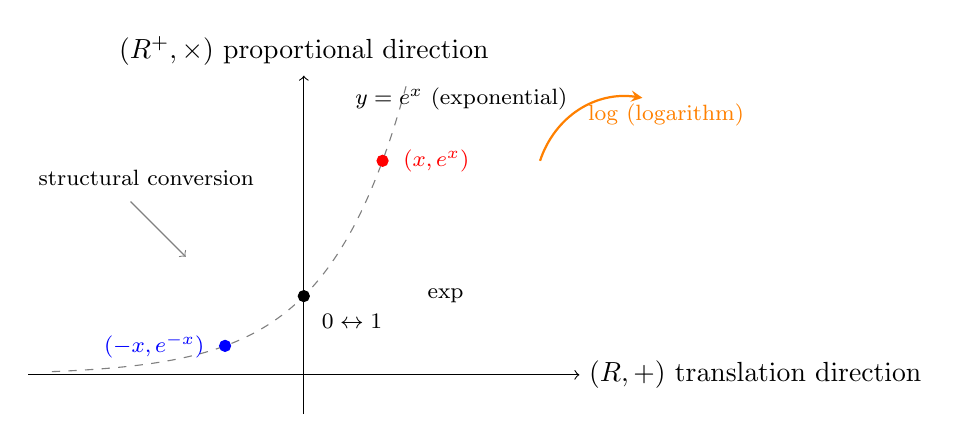
\begin{tikzpicture}[scale=1.0]
    \draw[->] (-3.5,0) -- (3.5,0) node[right] {$(\mathbb{R},+)$ translation direction};
    \draw[->] (0,-0.5) -- (0,3.8) node[above] {$(\mathbb{R}^+,\times)$ proportional direction};
    \draw[gray, dashed, domain=-3.2:1.3, samples=100] plot (\x, {exp(\x)});
    \node[font=\footnotesize] at (2.0, 3.5) {$y=e^x$ (exponential)};
    \node[font=\footnotesize] at (1.8, 1.0) {$\exp$};

    \filldraw[blue] (-1.0, {exp(-1.0)}) circle (2pt) node[left=4pt, font=\footnotesize] {$(-x,e^{-x})$};
    \filldraw[red] (1.0, {exp(1.0)}) circle (2pt) node[right=4pt, font=\footnotesize] {$(x,e^x)$};

    \draw[->, thick, >=stealth, orange] (3.0, {exp(1.0)}) to[bend left=40] (4.3, {exp(1.0)+0.8});
    \node[orange, font=\footnotesize] at (4.6, 3.3) {$\log$ (logarithm)};

    \node[font=\footnotesize] at (-2.0, 2.5) {structural conversion};
    \draw[->, gray, thin] (-2.2, 2.2) -- (-1.5, 1.5);

    \filldraw[black] (0,1) circle (2pt) node[below right=3pt, font=\footnotesize] {$0 \leftrightarrow 1$};
\end{tikzpicture}
\caption{The structural conversion function of the logarithm: the exponential map $\exp$ converts translations in the additive group into proportions in the multiplicative group; the logarithm $\log$ is its inverse map and converts the proportional direction into the translation direction. The multiplicative centre of symmetry $1$ corresponds to the additive centre of symmetry $0$.}
\label{fig:logarithm_converter}
\end{figure}
\section{\texorpdfstring{The period-determination spectrum of number-system extension}{The period-determination spectrum of number-system extension}}

\begin{theorem}[Correspondence between number-system extension and period-determination capability]\label{thm:number_system_period_criterion}
Let the time evolution of a system be given by a group action or a Hamiltonian flow. Then the number system required to describe the system and the period types it can determine or express stand in the following correspondence:
\[
\mathbb{Z} \Longrightarrow \text{can express discrete translation periods},
\]
\[
\mathbb{Q} \Longrightarrow \text{can express finite rotation periods},
\]
\[
\mathbb{R} \Longrightarrow \text{can express continuous translation periods and quasi-periods},
\]
\[
\mathbb{C} \Longrightarrow \text{can express rotation periods and double periods},
\]
\[
\mathbb{H} \Longrightarrow \text{can express three-dimensional rotation periods and non-commutative periods}.
\]
Each step of extension provides a new algebraic tool for the period-determination problems that could not be expressed in the preceding number system.
\end{theorem}

\begin{proof}
Combining the criterion theorems of the preceding sections level by level:
\begin{itemize}
    \item $\mathbb{Z}$: Theorem \ref{thm:integer_translation_criterion}---discrete translation periods can be determined.
    \item $\mathbb{Q}$: Theorem \ref{thm:rational_rotation_criterion}---finite rotation periods can be determined.
    \item $\mathbb{R}$: Theorem \ref{thm:real_quasi_period_criterion}---quasi-periods can be described.
    \item $\mathbb{C}$: Theorem \ref{thm:complex_finite_rotation_criterion} and Theorem \ref{thm:complex_double_period}---rotation periods and double periods are completely algebraised.
    \item $\mathbb{H}$: Theorem \ref{thm:quaternion_rotation_criterion} and Theorem \ref{thm:noncommutative_period}---three-dimensional rotation periods and non-commutative periods can be algebraised.
\end{itemize}
The extensions cannot be reversed level by level, because the closure newly added at each level precisely solves the period-determination problem that could not be expressed at the preceding level.
\end{proof}

\begin{theorem}[The correspondence between number-system extensions and the solvability of function equations]\label{thm:number_system_function_equation}
Each level of number-system extension makes exactly one class of function equation pass from `unsolvable' or `non-closed' to `solvable', with its group with periodic orbits becoming a group:
\begin{enumerate}[label=(\roman*)]
    \item $\mathbb{Z}$ makes the translation equation $f(x+a)=f(x)$ iterable in both directions, and the group with periodic orbits becomes the subgroup $a\mathbb{Z}$; the antiperiod equation $f(x+a)=-f(x)$ implies period doubling to $2a$.
    \item $\mathbb{Q}$ makes the scaling equation $f(qx)=f(x)$ iterable in both directions, and the group with periodic orbits becomes the subgroup $\langle q\rangle$; the commensurability criterion $\theta/(2\pi)\in\mathbb{Q}$ can be expressed exactly.
    \item $\mathbb{R}$ gives the continuous translation equation $f(x+t)=f(x)$ ($t\in\mathbb{R}$) a rigorous topological meaning, and the group with periodic orbits is a closed subgroup; the denseness of quasi-periodic orbits can be described rigorously.
    \item $\mathbb{C}$ makes the rotation equation $f(e^{i\theta}z)=f(z)$ algebraisable, and the group with periodic orbits is a subgroup of $U(1)$; finite rotation periods are characterised exactly by the unit-root equation $z^n=1$.
    \item $\mathbb{H}$ makes the three-dimensional rotation equation $f(qvq^{-1})=f(v)$ algebraisable, and the group with periodic orbits is a finite subgroup of $S^3\cong SU(2)$.
\end{enumerate}
\end{theorem}

\begin{proof}
Each item follows from the function-theoretic features of the preceding sections: $\mathbb{Z}$ from Theorem \ref{thm:translation_equation_Z}, $\mathbb{Q}$ from Theorem \ref{thm:scaling_equation_Q} and \ref{thm:rotation_equation_Q}, $\mathbb{R}$ from Theorem \ref{thm:translation_equation_R} and Proposition \ref{prop:quasi_period_R}, $\mathbb{C}$ from Theorem \ref{thm:rotation_equation_C} and Corollary \ref{cor:unit_root_C}, and $\mathbb{H}$ from Theorem \ref{thm:rotation_equation_H}.
\end{proof}

\begin{table}[htbp]
\centering
\caption{Solvability of three classes of function equation in each number system and the structure of the group with periodic orbits}
\label{tab:function_equation_solvability}
\small
\renewcommand{\arraystretch}{1.25}
\begin{tabular}{@{}>{\raggedright\arraybackslash}p{1.55cm}>{\raggedright\arraybackslash}p{3.6cm}>{\raggedright\arraybackslash}p{3.5cm}>{\raggedright\arraybackslash}p{5.05cm}@{}}
\toprule
\textbf{Number system} & \textbf{Translation $f(x+a)=f(x)$} & \textbf{Scaling $f(qx)=f(x)$} & \textbf{Rotation $f(e^{i\theta}z)=f(z)$} \\
\midrule
$\mathbb{N}$ & has solutions, period set not a group & non-invertible & no carrier \\
$\mathbb{Z}$ & group with periodic orbits $a\mathbb{Z}$ & non-invertible ($q^{-1}\notin\mathbb{Z}$) & no carrier \\
$\mathbb{Q}$ & group with periodic orbits $a\mathbb{Z}$ & group with periodic orbits $\langle q\rangle$ & commensurability criterion expressible \\
$\mathbb{R}$ & group with periodic orbits a closed subgroup & translation in the logarithmic domain & still no algebraic carrier \\
$\mathbb{C}$ & group with periodic orbits a closed subgroup & translation in the logarithmic domain & group with periodic orbits a subgroup of $U(1)$, exact via $z^n=1$ \\
$\mathbb{H}$ & group with periodic orbits a closed subgroup & translation in the logarithmic domain & group with periodic orbits a finite subgroup of $S^3\cong SU(2)$ \\
\bottomrule
\end{tabular}
\end{table}

\begin{table}[htbp]
\centering
\caption{Unified spectrum of number-system extension, determination requirements and period types}
\label{tab:number_system_period_spectrum}
\small
\begin{tabularx}{\textwidth}{@{}>{\raggedright\arraybackslash}p{1.6cm}
                  >{\raggedright\arraybackslash}X
                  >{\raggedright\arraybackslash}X
                  >{\raggedright\arraybackslash}X
                  >{\raggedright\arraybackslash}X@{}}
\toprule
\textbf{Number system} & \textbf{Determination requirement} & \textbf{Newly added closure} & \textbf{Period type} & \textbf{Conserved quantity} \\
\midrule
$\mathbb{N}$ & counting, indexing & no inverse operations & no period & --- \\
$\mathbb{Z}$ & two-directional extension of translation orbits & subtraction (additive inverse) & discrete translation period & momentum \\
$\mathbb{Q}$ & deciding commensurability & division (multiplicative inverse) & finite rotation period & angular momentum \\
$\mathbb{R}$ & denseness, continuity & completeness & quasi-period, continuous period & momentum, phase volume \\
$\mathbb{C}$ & algebraisation of rotation & imaginary unit $i$ & rotation period, double period & angular momentum \\
$\mathbb{H}$ & algebraisation of three-dimensional rotation & non-commutative multiplication & three-dimensional rotation period & three-dimensional angular momentum \\
\bottomrule
\end{tabularx}
\end{table}

\begin{corollary}[Period-diagnostic significance of number-system extension]\label{cor:number_system_diagnosis}
In the diagnosis of periodic mathematics, the hierarchy of number-system extension provides a determination tool:
\begin{enumerate}[label=(\roman*)]
    \item If a group action for the system can be constructed only on $\mathbb{Z}$, then the period types that can be determined are limited to discrete translation periods.
    \item If the system requires $\mathbb{Q}$ to express commensurability, then finite rotation periods can be determined.
    \item If the system requires $\mathbb{R}$ to express denseness and continuity, then quasi-periods can be described.
    \item If the system requires $\mathbb{C}$ to express the algebraisation of rotation and the period lattice, then rotation periods or double periods can be described.
    \item If the system requires $\mathbb{H}$ to express three-dimensional rotation, then three-dimensional rotation periods can be described.
\end{enumerate}
This diagnostic principle is a direct application of the theory of number-system extension to period determination.
\end{corollary}

\begin{proof}
Substituting item by item from Theorem \ref{thm:number_system_period_criterion} and Theorem \ref{thm:number_system_function_equation} gives---the required number system determines the period types that can be expressed or determined and the solvability of the function equations:
(i) If only $\mathbb{Z}$ can be used ($\mathbb{N}$ has no inverse operations and does not directly provide a tool for period determination, see Proposition \ref{prop:natural_no_inverse}), then $\mathbb{Z}$ corresponds to the discrete translation period, and the group with periodic orbits of the function equation $f(x+a)=f(x)$ is $a\mathbb{Z}$.
(ii) If $\mathbb{Q}$ is required, that is, multiplicative inverses are required in order to express commensurability $\theta/(2\pi)\in\mathbb{Q}$, then $\mathbb{Q}$ corresponds to the finite rotation period, and the group with periodic orbits of the function equation $f(qx)=f(x)$ is $\langle q\rangle$.
(iii) If $\mathbb{R}$ is required, that is, completeness is required in order to express denseness and continuity, then $\mathbb{R}$ corresponds to the quasi-period, and the group with periodic orbits of the continuous translation equation is a closed subgroup.
(iv) If $\mathbb{C}$ is required, that is, algebraic closure is required in order to give the complete solution set of $z^n = 1$ and the period lattice $\Lambda$, then $\mathbb{C}$ corresponds to the rotation period or the double period, and the group with periodic orbits of the rotation equation is a subgroup of $U(1)$.
(v) If $\mathbb{H}$ is required, that is, non-commutative multiplication is required in order to express three-dimensional rotation, then $\mathbb{H}$ corresponds to the three-dimensional rotation period, and the group with periodic orbits of the three-dimensional rotation equation is a finite subgroup of $SU(2)$.
\end{proof}

\begin{figure}[htbp]
\centering
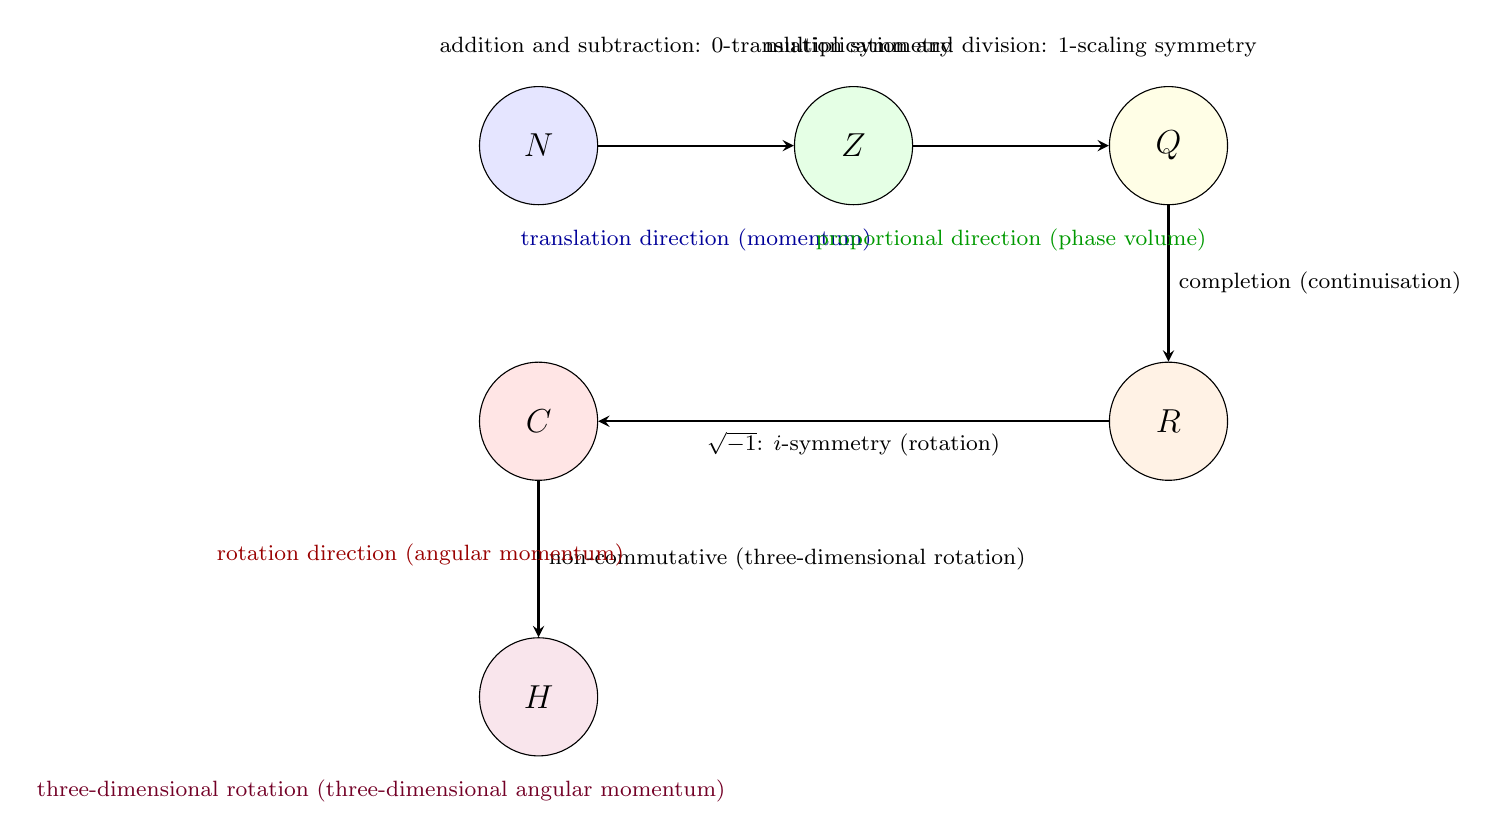
\begin{tikzpicture}[>=stealth, node distance=2.8cm and 3.2cm,
    ns/.style={draw, circle, minimum size=1.5cm, inner sep=0pt, font=\large\bfseries},
    arrow/.style={->, thick, >=stealth, font=\footnotesize}]

    \node[ns, fill=blue!10] (N) at (0,0) {$\mathbb{N}$};
    \node[ns, fill=green!10] (Z) at (4,0) {$\mathbb{Z}$};
    \node[ns, fill=yellow!10] (Q) at (8,0) {$\mathbb{Q}$};
    \node[ns, fill=orange!10] (R) at (8,-3.5) {$\mathbb{R}$};
    \node[ns, fill=red!10] (C) at (0,-3.5) {$\mathbb{C}$};
    \node[ns, fill=purple!10] (H) at (0,-7.0) {$\mathbb{H}$};

    \draw[arrow] (N) -- (Z) node[midway, above=1cm] {addition and subtraction: $0$-translation symmetry};
    \draw[arrow] (Z) -- (Q) node[midway, above=1cm] {multiplication and division: $1$-scaling symmetry};
    \draw[arrow] (Q) -- (R) node[midway, right] {completion (continuisation)};
    \draw[arrow] (R) -- (C) node[midway, below, sloped] {$\sqrt{-1}$: $i$-symmetry (rotation)};
    \draw[arrow] (C) -- (H) node[midway, right] {non-commutative (three-dimensional rotation)};

    \node[font=\footnotesize, text=blue!60!black] at (2, -1.2) {translation direction (momentum)};
    \node[font=\footnotesize, text=green!60!black] at (6, -1.2) {proportional direction (phase volume)};
    \node[font=\footnotesize, text=red!60!black] at (-1.5, -5.2) {rotation direction (angular momentum)};
    \node[font=\footnotesize, text=purple!60!black] at (-2, -8.2) {three-dimensional rotation (three-dimensional angular momentum)};
\end{tikzpicture}
\caption{The path of number-system extension and the progression of the transformation hierarchy (chapter summary diagram). Each step of extension establishes a new centre of symmetry by introducing a new inverse operation, thereby producing a new type of transformation: subtraction ($0$-symmetry) makes translation two-directional; division ($1$-symmetry) introduces scaling---repeated translation produces scaling; the imaginary unit ($i$-symmetry) introduces rotation---repeated scaling produces rotation; non-commutative multiplication introduces three-dimensional rotation. The logarithm converts scaling into translation, and the complex logarithm converts rotation into translation; in the logarithmic domain the three transformations are unified as addition. For the local diagram of $\mathbb{N}\to\mathbb{Z}\to\mathbb{Q}$, see Section \ref{prop:integer_symmetry_direction_period} and its Figure \ref{fig:symmetry_centre_emergence}.}
\label{fig:number_extension}
\end{figure}
\section*{Seven-theme comparison table for this chapter}

\begin{center}
\renewcommand{\arraystretch}{1.3}
\begin{tabular}{>{\centering\arraybackslash}p{2.2cm}>{\centering\arraybackslash}p{10.5cm}}
\toprule
Theme & Corresponding content in this chapter \\
\midrule
Translation & the translation period criterion for the integers (Theorem \ref{thm:integer_translation_criterion}) and discrete translation periods (Corollary \ref{cor:integer_discrete_translation}); the logarithm converting the proportional direction into the translation direction (Theorem \ref{thm:logarithm_conversion}); the groups with periodic orbits of the translation equation (Theorems \ref{thm:translation_equation_Z}, \ref{thm:translation_equation_R}) \\
Scaling & the proportional direction of the rationals (Proposition \ref{prop:rational_direction_period}) and the taking-the-inverse involution $\sigma_1$ (Definition \ref{def:rational_involution}); conversion of conserved quantities under the logarithmic isomorphism (Theorem \ref{thm:log_isomorphism_conservation}); the group with periodic orbits of the scaling equation (Theorem \ref{thm:scaling_equation_Q}) \\
Rotation & algebraisation of complex rotation (Theorem \ref{thm:complex_rotation_algebraization}) and the criterion for finite rotation periods (Theorem \ref{thm:complex_finite_rotation_criterion}); three-dimensional rotation by quaternions (Theorem \ref{thm:quaternion_rotation_criterion}); the groups with periodic orbits of the rotation equation (Theorems \ref{thm:rotation_equation_C}, \ref{thm:rotation_equation_H}) \\
Conservation & the closure of the operations of each number system (construction of the integers \ref{def:integer_construction}; algebraic closure of the complex numbers \ref{prop:complex_algebraically_closed}); multiplicativity of the quaternion norm and Casimir conservation (Proposition \ref{prop:quaternion_direction_period}) \\
Symmetry & the emergence of the centres of symmetry $0,1,i$: the additive involution (integers), the multiplicative involution $\sigma_1$ (rationals) and the $i$-involution (complex numbers, Definition \ref{def:complex_i_involution}) \\
Closure & two-step closure of an involution ($\sigma^2=\mathrm{id}$); finite rotation period $\Leftrightarrow$ closure of the roots of unity (Theorem \ref{thm:complex_finite_rotation_criterion}) \\
Period & the correspondence between number-system extension and period-determination capability (Theorem \ref{thm:number_system_period_criterion}), the correspondence between number-system extension and the solvability of function equations (Theorem \ref{thm:number_system_function_equation}) and the period-determination spectrum (Table \ref{tab:number_system_period_spectrum}): discrete translation / finite rotation / quasi-period / double period / non-commutative period \\
\bottomrule
\end{tabular}
\end{center}

\section*{Exercises}

\begin{enumerate}[leftmargin=3em, label=\textbf{Exercise \arabic*}]
    \item Prove the three assertions about the absence of inverse operations in the natural numbers in Proposition \ref{prop:natural_no_inverse}:
    under what conditions subtraction, division and root extraction have a natural-number solution, and under what conditions they have none.
    Further explain why the natural numbers cannot form a group, and explain the conclusion of Corollary \ref{cor:natural_period}
    that `the determination of discrete translation periods requires at least the group structure of $\mathbb{Z}$'.

    \item Fill in the details of the proof of the well-definedness of multiplication in Proposition \ref{prop:integer_well_defined},
    and verify that addition, multiplication, the zero element and inverses in the construction of the integers \ref{def:integer_construction}
    really do not depend on the choice of representative of the equivalence class. Finally explain why the additive group of
    $\mathbb{Z}$ is the minimal algebraic structure that enables translation orbits to be extended in both directions and hence
    their closure to be determined (see Remark \ref{rem:integer_makes_translation_invertible}).

    \item In $\mathbb{Z}/12\mathbb{Z}$ compute the orders of the elements $[3]$, $[4]$, $[5]$ and $[7]$,
    and verify the formula of Lemma \ref{lem:order_cyclic_subgroup_ch2}
    \[
    \operatorname{ord}([T])=\frac{12}{\gcd(T,12)}.
    \]
    Point out which elements are generators of $\mathbb{Z}/12\mathbb{Z}$.
    If $12$ is understood as the period of the Earthly Branches, explain how the orders of these elements correspond to the sub-period structure within the period $12$.

    \item Prove the assertion in Theorem \ref{thm:integer_translation_criterion} that a translation orbit
    degenerates to a single point in $\mathbb{Z}/m\mathbb{Z}$ if and only if $T\equiv0\pmod m$.
    Also construct a concrete example: take $m=12$, $T\neq0$, but the minimal period of the orbit in $\mathbb{Z}/12\mathbb{Z}$
    is strictly less than $12$. Compute the length of this orbit.

    \item Verify that $\mathbb{Q}$ forms a field (Proposition \ref{prop:rational_field}),
    and prove that the taking-the-inverse map
    \[
    \sigma_1:\mathbb{Q}^{\times}\to\mathbb{Q}^{\times},\qquad
    \sigma_1(x)=x^{-1}
    \]
    is an automorphism of the multiplicative group and an involution, with fixed-point set $\{1,-1\}$
    (see Definition \ref{def:rational_involution} and Proposition \ref{prop:rational_involution_properties}).
    Explain how $\sigma_1$ interchanges the operation of `enlargement' with the operation of `shrinkage'.

    \item Prove Theorem \ref{thm:rational_rotation_criterion}:
    if $\theta/(2\pi)=p/q$ is a rational number in lowest terms, then the rotation orbit
    \[
    \mathcal{O}(z_0;\theta)=\{z_0e^{in\theta}\mid n\in\mathbb{Z}\}
    \]
    contains exactly $q$ points and has period $q$;
    if $\theta/(2\pi)\notin\mathbb{Q}$, then the orbit does not close.
    Further explain why the criterion of `commensurability' itself requires $\mathbb{Q}$
    in order to be expressed exactly, whereas $\mathbb{R}$ can describe only its limits and denseness.

    \item Prove that the completeness of the reals closes the root operation (Theorem \ref{thm:real_root_closure}),
    and give an equation that has no solution in $\mathbb{Q}$ but has one in $\mathbb{R}$.
    Then explain why the description of the denseness of quasi-periodic orbits must rely on the completeness of $\mathbb{R}$
    (see Proposition \ref{prop:quasi_period_R} and Theorem \ref{thm:real_quasi_period_criterion}).

    \item Verify that the set of $n$-th roots of unity
    \[
    \{\zeta_k=e^{2\pi ik/n}\mid k=0,1,\dots,n-1\}
    \]
    forms the cyclic group $C_n$ under complex multiplication (Theorem \ref{thm:complex_finite_rotation_criterion}).
    Write out all the roots of unity for $n=8$ explicitly, and explain their correspondence with the rotation period $C_8$.
    Finally explain why $\mathbb{C}$ is the minimal field extension that makes the rotation equation algebraisable
    (see Remark \ref{rem:complex_makes_rotation_algebraic}).

    \item Prove that the map
    \[
    \sigma_i:\mathbb{C}^{\times}\to\mathbb{C}^{\times},\qquad
    \sigma_i(z)=iz^{-1}
    \]
    is an involution and find its fixed points. Writing $z$ in polar form $z=re^{i\varphi}$,
    explain that $\sigma_i$ comprises simultaneously the taking of the reciprocal of the modulus and a reflection of the argument about the $\pi/4$ direction
    (see Definition \ref{def:complex_i_involution} and Proposition \ref{prop:complex_i_involution_properties}).

    \item Prove that the quaternion unit sphere
    \[
    S^3=\{q\in\mathbb{H}\mid |q|=1\}
    \]
    through the conjugation action
    \[
    \rho_q(v)=qvq^{-1},\qquad v\in\operatorname{Im}(\mathbb{H})\cong\mathbb{R}^3
    \]
    realises three-dimensional rotations, and that the map
    \[
    \Pi:S^3\to SO(3),\qquad q\mapsto\rho_q
    \]
    is a double covering with kernel $\{\pm1\}$ (Theorem \ref{thm:quaternion_rotation_criterion}).
    Then give an example showing that rotations about different axes do not commute in general (Theorem \ref{thm:noncommutative_period}).

    \item Verify that the logarithmic isomorphism
    \[
    \ln:(\mathbb{R}^+,\times)\to(\mathbb{R},+)
    \]
    maps the multiplicative centre of symmetry $1$ to the additive centre of symmetry $0$,
    and converts conserved quantities under the proportional direction into conserved quantities under the translation direction
    (see Theorem \ref{thm:logarithm_conversion}, Theorem \ref{thm:log_isomorphism_conservation}
    and Proposition \ref{prop:log_symmetry_centre_unification}).
    Taking $f(x)=\sin(2\pi\log_q x)$ as an example, verify that $f(qx)=f(x)$,
    and write down its translation-period form in the variable $t=\ln x$.

    \item Synthesis question: using Theorem \ref{thm:number_system_period_criterion}
    and Table \ref{tab:number_system_period_spectrum}, explain why
    `discrete translation period', `finite rotation period', `double period' and `three-dimensional rotation period'
    require at least $\mathbb{Z}$, $\mathbb{Q}$, $\mathbb{C}$ and $\mathbb{H}$ respectively.
    Construct a counterexample showing that planar rotation periods cannot be algebraised in $\mathbb{R}$.
    Then discuss: if a system is defined only on $\mathbb{N}$, can its translation period be determined?
    If not, to which level must the number system be extended at least? Give reasons.

    \item Write down, in the logarithmic coordinates $(\ln|z|,\arg z)$, the matrix of multiplication by $b=u+iv$,
    \[
    M_b=\begin{pmatrix}u&-v\\ v&u\end{pmatrix},
    \]
    and explain the meaning of its off-diagonal entries $\pm v$ (Theorem \ref{thm:power_matrix_log_coordinates}).
    Taking $b=1+i$ and $z_0=2e^{i\pi/4}$, compute the logarithmic coordinates of $z_0^{b}$,
    and identify which term comes from `rotation coupled into scaling' and which from `scaling coupled into rotation'
    (see Example \ref{ex:power_coupling_example}).
    Finally explain why the assertion that `the power sequence $\{z b^n\}$ lies on an equiangular spiral' presupposes $v\neq0$,
    and why the criterion degenerates, when $|b|=1$, into the dichotomy of closure and denseness on a circle
    (see Corollary \ref{cor:spiral_criterion} and Theorem \ref{thm:rational_rotation_criterion});
    and state which convergence conditions the single-valuedness of $z^b$ requires (Property \ref{prop:power_preconditions}).
\end{enumerate}

